\documentclass[12pt,letterpaper]{article}
\usepackage[T1]{fontenc}
\usepackage{mathptmx}
\usepackage{courier}
\usepackage[letterpaper,margin=1in]{geometry}
\usepackage{amsmath,amssymb,amsthm}
\usepackage{microtype}
\usepackage{booktabs}
\usepackage{array}
\usepackage{enumitem}
\usepackage{tikz}
\usetikzlibrary{arrows.meta,positioning}
\usepackage[hidelinks]{hyperref}

\tikzset{
  vx/.style={circle,draw,fill=white,inner sep=1.2pt,minimum size=17pt,font=\footnotesize},
  bx/.style={circle,draw,fill=blue!12,inner sep=1.2pt,minimum size=17pt,font=\footnotesize},
  rx/.style={circle,draw,fill=red!14,inner sep=1.2pt,minimum size=17pt,font=\footnotesize},
  ar/.style={-{Stealth[length=2.2mm]},thick},
  mapto/.style={-{Stealth[length=3mm]},very thick}
}

\numberwithin{equation}{section}

\theoremstyle{plain}
\newtheorem{theorem}{Theorem}[section]
\newtheorem{proposition}[theorem]{Proposition}
\newtheorem{lemma}[theorem]{Lemma}
\newtheorem{corollary}[theorem]{Corollary}
\theoremstyle{definition}
\newtheorem{definition}[theorem]{Definition}
\newtheorem{example}[theorem]{Example}
\newtheorem{remark}[theorem]{Remark}
\newtheorem{question}[theorem]{Question}

\newcommand{\Z}{\mathbb{Z}}
\newcommand{\C}{\mathbb{C}}
\newcommand{\R}{\mathbb{R}}
\newcommand{\Q}{\mathbb{Q}}
\newcommand{\Fq}{\mathbb{F}}
\newcommand{\cO}{\mathcal{O}}
\newcommand{\pmat}[4]{\bigl(\begin{smallmatrix}#1&#2\\#3&#4\end{smallmatrix}\bigr)}
\newcommand{\Gh}{\widehat{G}}
\newcommand{\Th}{\widehat{T}}
\newcommand{\act}[2]{{}^{#1}\!#2}          % action of #1 on #2
\newcommand{\fr}{\mathcal{F}}             % free group
\newcommand{\rel}{\mathcal{R}}            % relation subgroup
\newcommand{\LG}{{}^{L}G}
\DeclareMathOperator{\Hom}{Hom}
\DeclareMathOperator{\Aut}{Aut}
\DeclareMathOperator{\Int}{Int}
\DeclareMathOperator{\Out}{Out}
\DeclareMathOperator{\Cent}{Cent}
\DeclareMathOperator{\Stab}{Stab}
\DeclareMathOperator{\Gal}{Gal}
\DeclareMathOperator{\Cay}{Cay}
\DeclareMathOperator{\GL}{GL}
\DeclareMathOperator{\SL}{SL}
\DeclareMathOperator{\PGL}{PGL}
\DeclareMathOperator{\Ind}{Ind}
\DeclareMathOperator{\diag}{diag}
\DeclareMathOperator{\val}{val}
\DeclareMathOperator{\infl}{inf}
\DeclareMathOperator{\res}{res}
\newcommand{\Nm}{\mathrm{N}_{E/F}}

\title{Notes on the inflation-restriction sequence\\ in non-abelian cohomology\\[4pt]
\large Draft 1. Corrected and expanded version}
\author{David Joyner\thanks{This note corrects and expands an undated,
unpublished manuscript of the same title (file \texttt{infres.tex}, written
in \AmS-\TeX\ while the author was at the U.S.\ Naval Academy). Draft~1 of
this revision was prepared on November 26, 2026.}\\
\texttt{wdjoyner@gmail.com}
\and Claude\thanks{An AI system developed by Anthropic (model Claude
Fable~5.2). Its contributions are described in the Acknowledgments.}}
\date{Original draft: undated (1990s). Corrected and expanded draft: 2026}

\begin{document}
\maketitle

\begin{abstract}
The second author of this note is an AI system (Claude, by Anthropic),
which revised, corrected and expanded the first author's original
manuscript; another AI system (Gemini, by Google) acted as referee. See
the Acknowledgments for details.

Let $1\to N\to W\to\Gamma\to 1$ be an extension of groups with $N$ abelian,
for example the relative Weil group $W_{E/F}$ of a finite Galois extension
$E/F$ of $p$-adic fields, with $N=E^\times$ and $\Gamma=\Gal(E/F)$. Let $A$
be a group on which $\Gamma$ acts, for example the complex dual group of a
reductive group over $F$. We give a self-contained account of the
non-abelian inflation-restriction sequence
\[
1\to H^1(\Gamma,A)\to H^1(W,A)\to H^1(N,A)^\Gamma ,
\]
and we determine the image of the restriction map. A homomorphism
$\phi:N\to A$ whose conjugacy class is $\Gamma$-invariant is the restriction
of a $1$-cocycle of $W$ if and only if a class $\partial\phi$ is neutral, where
$\partial\phi$ lies in Springer's non-abelian $H^2$ of $\Gamma$ with
coefficients in the \emph{centralizer} of $\phi(N)$ in $A$. The fibers of the
restriction map are described by twisting. We show by examples that the
centralizer cannot be replaced by $A$. Finally we recast the criterion in
terms of voltage and gain graphs: the Cayley graph of $W$ is the derived
graph of a voltage assignment on the Cayley graph of $\Gamma$, and $\phi$
extends exactly when a gain function on the Cayley graph of $\Gamma$ has the
holonomy prescribed by $\phi$ around each defining relator of $\Gamma$.
\end{abstract}

\tableofcontents

\section{Introduction}\label{sec:intro}

\subsection{Setting and motivation}

Let $E/F$ be a finite Galois extension of $p$-adic fields, with Galois
group $\Gamma=\Gal(E/F)$. Let $W_F$ and $W_E$ be the absolute Weil groups
and let $W_E^c$ be the closure of the commutator subgroup of $W_E$. The
relative Weil group $W=W_{E/F}=W_F/W_E^c$ fits into the short exact sequence
\begin{equation}\label{eq:weil}
1\longrightarrow E^{\times}\overset{i}{\longrightarrow} W
\overset{p}{\longrightarrow}\Gamma\longrightarrow 1 ,
\end{equation}
where $E^\times$ is identified with $W_E/W_E^c$, the maximal abelian
Hausdorff quotient of $W_E$, by the reciprocity map of local class field
theory.

Let $G$ be a connected reductive group over $F$ which splits over $E$, and
let $\Gh=\Gh(\C)$ be its complex dual group. The group $\Gamma$ acts on
$\Gh$, and the action is trivial exactly when $G$ is an inner form of a
split group. Through $p$, the group $W$ acts on $\Gh$, and the subgroup
$E^\times$ acts trivially because $p\circ i$ is trivial. Langlands
parameters of $G$ whose restriction to $W_E$ has abelian image give classes
in the cohomology set $H^1(W,\Gh)$ (Section~\ref{sec:langlands}). It is
therefore natural to ask how $H^1(W,\Gh)$ is built from cohomology of
$\Gamma$ and of $E^\times$.

For an abelian coefficient group the answer is the classical
inflation-restriction sequence \cite[Ch.~VII, \S6]{Se} together with the
transgression map of Hochschild and Serre \cite{HS}. The purpose of this
note is to work out the non-abelian analog. The arguments are exercises in
cohomology, but the result has some content: the obstruction to extending a
homomorphism $\phi:E^\times\to\Gh$ to a parameter does not live in a
cohomology set of $\Gh$. It lives in a cohomology set of the centralizer of
the image of $\phi$.

\subsection{Results}

Nothing in the argument uses the arithmetic of~\eqref{eq:weil}, so we work
with an arbitrary extension of groups
\[
1\longrightarrow N\overset{i}{\longrightarrow} W
\overset{p}{\longrightarrow}\Gamma\longrightarrow 1 ,\qquad N\ \text{abelian},
\]
and an arbitrary group $A$ with an action of $\Gamma$. The main results are
the following.

\begin{itemize}[itemsep=2pt]
\item \emph{Theorem~\ref{thm:exact}.} The sequence of pointed sets
$1\to H^1(\Gamma,A)\to H^1(W,A)\to H^1(N,A)^\Gamma$ is exact, and inflation
is injective. Here $H^1(N,A)$ is the set of conjugacy classes of
homomorphisms $N\to A$.
\item \emph{Theorem~\ref{thm:main}.} Let $\phi:N\to A$ be a homomorphism
whose class is $\Gamma$-invariant, and let $C_\phi$ be the centralizer of
$\phi(N)$ in $A$. There is a class $\partial\phi$ in Springer's set
$H^2(\Gamma,C_\phi,\kappa_\phi)$ such that $\phi$ is the restriction of a
$1$-cocycle of $W$ if and only if $\partial\phi$ is neutral. Equivalently,
$\phi$ extends to a morphism from the extension $W$ to the stabilizer
extension $E_\phi$ of $\Gamma$ by $C_\phi$.
\item \emph{Proposition~\ref{prop:fiber}.} The fiber of the restriction map
through the class of a cocycle $f$ is in bijection with
$H^1(\Gamma,C_\phi)$, where $\phi=f|_N$ and $\Gamma$ acts on $C_\phi$
through $f$.
\item \emph{Corollary~\ref{cor:central}.} When $\phi$ takes values in the
center of $A$, the class $\partial\phi$ is the class of
$(\phi\circ\sigma)^{-1}$ in $H^2(\Gamma,A,\overline{\alpha})$, where $\sigma$
is a factor set of $W$. For abelian $A$ this is the classical five-term
sequence.
\item \emph{Theorem~\ref{thm:graph}.} Choose generators $\overline{S}$ of
$\Gamma$ and lifts of them to $W$. Then $\phi$ is the restriction of a
cocycle if and only if there is a $\Gamma$-equivariant gain function on the
Cayley graph $\Cay(\Gamma,\overline{S})$ whose net gain around each
defining relator of $\Gamma$ is the image under $\phi$ of the net
$N$-voltage of that relator. For cyclic $\Gamma$ this is a single
``twisted norm'' equation (Corollary~\ref{cor:cyclic}).
\end{itemize}

A detailed running example, the Weil group of $\Q_3(i)/\Q_3$ with
coefficients in $\C^\times$ and in $\SL_2(\C)$, is carried through the
whole note: Examples~\ref{ex:run1}, \ref{ex:run2}, \ref{ex:run3},
\ref{ex:run4} and~\ref{ex:run5}, at the ends of
Sections~\ref{sec:background} to~\ref{sec:langlands}. In it every object
of the note is computed explicitly. Three shorter examples recur as well: a toy extension of $\Z/2$ by
$\Z/4$, which is either the dihedral or the quaternion group of order~$8$
(Examples~\ref{ex:toy}, \ref{ex:toy-noeq}, \ref{ex:toy-obstruction},
\ref{ex:toy-graph}); the norm-one torus of a quadratic extension
(Examples~\ref{ex:torus1}, \ref{ex:torus2}); and dihedral parameters with
values in $\SL_2(\C)$ (Example~\ref{ex:dihedral}).

\subsection{Standing assumptions and scope}\label{ss:scope}

\begin{itemize}[itemsep=2pt]
\item \emph{$N$ is abelian.} This is used in Lemma~\ref{lem:factor} and to
know that $\phi(N)$ lies in the center of $C_\phi$. Theorem~\ref{thm:exact}
does not need it.
\item \emph{Groups are discrete} in Sections~\ref{sec:background}
to~\ref{sec:graph}. Section~\ref{sec:langlands} shows that every statement
holds verbatim for continuous cocycles when $N$ is open in $W$, which is
the case for $W_{E/F}$.
\item \emph{In statements about $W_{E/F}$ we assume $E\neq F$} whenever we
say that the extension~\eqref{eq:weil} does not split.
Examples~\ref{ex:weil-quad}, \ref{ex:torus1}, \ref{ex:torus2}
and~\ref{ex:dihedral} assume $[E:F]=2$, and the running example is the
unramified quadratic extension of $\Q_3$.
\item No Weil--Deligne group, and no condition of semisimplicity or
relevance, enters this note. Its subject is the cohomology set
$H^1(W_{E/F},\Gh)$, which contains the relevant set of Langlands parameters
(Remark~\ref{rem:parameters}).
\end{itemize}

\subsection{What is proved here and what is cited}

\begin{center}
\begin{tabular}{@{}p{0.47\textwidth}p{0.47\textwidth}@{}}
\toprule
Proved in this note & Cited \\
\midrule
Lemmas \ref{lem:factor}, \ref{lem:semidirect}, \ref{lem:ext-class},
\ref{lem:twist}, \ref{lem:actions}, \ref{lem:restrict}, \ref{lem:T} &
Structure of $W_{E/F}$: facts (W1)--(W3) of \S\ref{ss:weil}
\cite{Ta,AT} \\
Theorems \ref{thm:exact}, \ref{thm:main}, \ref{thm:graph} &
$H^2(\Z/2,C)$ for abelian $C$ (Example~\ref{ex:H2}) \cite{Se} \\
Propositions \ref{prop:welldef}, \ref{prop:fiber}, \ref{prop:derived},
\ref{prop:cont} &
Langlands' correspondence for tori (Example~\ref{ex:torus2}, comparison
only) \cite{La} \\
Corollaries \ref{cor:central}, \ref{cor:cyclic} &
Coverings are harmonic morphisms (Remark~\ref{rem:harmonic}) \cite{BN} \\
 & Structure of $\Q_3(i)^\times$ and its norm group
(Example~\ref{ex:run1}(a),(b)) \cite{Se} \\
All computations in the examples & \\
\bottomrule
\end{tabular}
\end{center}

\noindent The finite examples, and the main results for twenty small
extensions and coefficient groups, were also checked by exhaustive
computer enumeration; see the script in the folder \texttt{verification}
of the repository named in the Acknowledgments.

\subsection{Related literature}

The definitions of non-abelian $H^0$ and $H^1$, twisting, and the exact
sequence of Theorem~\ref{thm:exact} are in Serre's book
\cite[Ch.~I, \S5]{Se2}. The second cohomology set with coefficients in a
non-abelian group, defined relative to a ``kernel'' (or ``band''), and its
neutral classes are due to Springer \cite{Spr} and Giraud \cite{Gi}; see
also Borovoi \cite{Bor}. The underlying obstruction theory for group
extensions with non-abelian kernel goes back to Eilenberg and Mac~Lane; see
\cite[Ch.~IV, \S8]{ML}. Theorem~\ref{thm:main} is an instance of that
theory and is presumably known to experts, but the authors have not found it
stated in the form needed here. The abelian case is in \cite{HS}. For Weil
groups see \cite{Ta} and \cite[Ch.~XV]{AT}, and for $L$-groups and
parameters see \cite{Bo}. Voltage graphs and derived graphs are treated in
\cite{GT}, gain graphs in \cite{Za}, and harmonic morphisms of graphs in
\cite{BN}.

\subsection{Organization}

Section~\ref{sec:background} collects background: factor sets, the relative
Weil group, non-abelian $H^1$, and Springer's $H^2$.
Section~\ref{sec:infres} treats inflation and restriction.
Section~\ref{sec:obstruction} constructs the obstruction class and proves
the main theorem. Section~\ref{sec:graph} gives the graph-theoretic
formulation. Section~\ref{sec:langlands} discusses topology and Langlands
parameters, and Section~\ref{sec:questions} lists some questions. Each of
Sections~\ref{sec:background} to~\ref{sec:langlands} ends with the
corresponding part of the running example. A glossary is at the end.

\section{Background and conventions}\label{sec:background}

Throughout, $1\to N\overset{i}{\to}W\overset{p}{\to}\Gamma\to1$ is an exact
sequence of groups with $N$ abelian. We identify $N$ with $i(N)$. The group
$N$ is written multiplicatively.

\subsection{Extensions and factor sets}

Since $N$ is abelian and normal, $W$ acts on $N$ by conjugation and $N$
acts trivially. Hence $\Gamma$ acts on $N$: for $g\in\Gamma$ and $x\in N$,
\begin{equation}\label{eq:actN}
\act{g}{x}=wxw^{-1}\qquad\text{for any } w\in W \text{ with } p(w)=g .
\end{equation}

\begin{definition}\label{def:section}
A \emph{section} of $p$ is a map of sets $s:\Gamma\to W$ with $p\circ s$
the identity and $s(1)=1$. Its \emph{factor set} is the map
$\sigma:\Gamma\times\Gamma\to W$,
\begin{equation}\label{eq:sigma}
\sigma(g,h)=s(g)s(h)s(gh)^{-1}.
\end{equation}
\end{definition}

No compatibility of $s$ with conjugation is assumed.\footnote{The original
manuscript used the inverse convention
$\sigma(g,h)=s(gh)s(h)^{-1}s(g)^{-1}$. The convention~\eqref{eq:sigma} is
the usual one for factor sets.}

\begin{lemma}\label{lem:factor}
Let $s$ be a section with factor set $\sigma$.
\begin{enumerate}[label=\textup{(\roman*)},itemsep=1pt]
\item $\sigma$ takes values in $N$, and $\sigma(g,1)=\sigma(1,g)=1$.
\item Every element of $W$ can be written uniquely as $x\,s(g)$ with
$x\in N$ and $g\in\Gamma$, and
\begin{equation}\label{eq:mult}
\bigl(x\,s(g)\bigr)\bigl(y\,s(h)\bigr)=x\cdot\act{g}{y}\cdot\sigma(g,h)\,s(gh).
\end{equation}
\item For all $g,h,k\in\Gamma$,
\begin{equation}\label{eq:2coc}
\act{g}{\sigma(h,k)}\;\sigma(g,hk)=\sigma(g,h)\,\sigma(gh,k).
\end{equation}
Thus $\sigma$ is a $2$-cocycle of $\Gamma$ with values in the
$\Gamma$-module $N$.
\item If $s'=\eta s$ is another section, where $\eta:\Gamma\to N$ and
$\eta(1)=1$, then its factor set is
$\sigma'(g,h)=\eta(g)\,\act{g}{\eta(h)}\,\eta(gh)^{-1}\sigma(g,h)$. Hence
the class $[\sigma]\in H^2(\Gamma,N)$ does not depend on $s$. It is trivial
if and only if the extension splits, that is, if and only if $p$ has a
section which is a homomorphism.
\end{enumerate}
\end{lemma}

\begin{proof}
(i) Applying $p$ to~\eqref{eq:sigma} gives $gh(gh)^{-1}=1$, so
$\sigma(g,h)\in\ker p=N$. The normalization follows from $s(1)=1$.

(ii) For $w\in W$ put $g=p(w)$ and $x=ws(g)^{-1}\in N$. Uniqueness is
clear. By~\eqref{eq:actN} and~\eqref{eq:sigma},
$x\,s(g)\,y\,s(h)=x\,\act{g}{y}\,s(g)s(h)=x\,\act{g}{y}\,\sigma(g,h)s(gh)$.

(iii) Compute $s(g)s(h)s(k)$ in two ways:
\begin{align*}
\bigl(s(g)s(h)\bigr)s(k)&=\sigma(g,h)\,s(gh)s(k)=\sigma(g,h)\,\sigma(gh,k)\,s(ghk),\\
s(g)\bigl(s(h)s(k)\bigr)&=s(g)\,\sigma(h,k)\,s(hk)
=\act{g}{\sigma(h,k)}\,s(g)s(hk)=\act{g}{\sigma(h,k)}\,\sigma(g,hk)\,s(ghk).
\end{align*}

(iv) We have
\[
s'(g)s'(h)=\eta(g)s(g)\,\eta(h)s(h)
=\eta(g)\,\act{g}{\eta(h)}\,\sigma(g,h)\,s(gh)
\]
and $s(gh)=\eta(gh)^{-1}s'(gh)$. So $\sigma'$ and $\sigma$ differ by a
coboundary. If $s$ is a homomorphism then $\sigma=1$. Conversely, if
$[\sigma]$ is trivial then some $\sigma'$ equals $1$, and then $s'$ is a
homomorphism.
\end{proof}

\begin{example}[The toy extensions]\label{ex:toy}
Let $N=\langle\rho\rangle$ be cyclic of order $4$ and $\Gamma=\{1,\tau\}$,
with $\act{\tau}{\rho}=\rho^{-1}$. For $a\in N^\Gamma=\{1,\rho^2\}$ let
\[
W_a=\langle \rho, s \mid \rho^4=1,\ s\rho s^{-1}=\rho^{-1},\ s^2=a\rangle .
\]
This is a group of order $8$ containing $N$ with quotient $\Gamma$. Take
the section $s(\tau)=s$. Its factor set has one non-trivial value,
$\sigma(\tau,\tau)=s^2=a$. The group $W_1$ is the dihedral group $D_4$ of
order $8$, a split extension. The group $W_{\rho^2}$ is the quaternion
group $Q_8=\{\pm1,\pm i,\pm j,\pm k\}$, with $\rho=i$ and $s=j$. Every
element of $Q_8$ outside $N$ has order $4$, so this extension does not
split and $[\sigma]\neq0$. In fact $H^2(\Gamma,N)$ has two elements
(Example~\ref{ex:H2}), so these are all the extensions of $\Gamma$ by $N$
with this action.
\end{example}

\subsection{The relative Weil group}\label{ss:weil}

For $W=W_{E/F}$ we use the following standard facts
\cite[\S1]{Ta}, \cite[Ch.~XV]{AT}.

\begin{enumerate}[label=\textup{(W\arabic*)},itemsep=1pt]
\item The sequence~\eqref{eq:weil} is exact, with $E^\times\cong W_E/W_E^c$
by the reciprocity map.
\item The action~\eqref{eq:actN} of $\Gamma$ on $E^\times$ is the Galois
action.
\item The class $[\sigma]\in H^2(\Gamma,E^\times)$ is the fundamental class
$u_{E/F}$ of local class field theory. The group $H^2(\Gamma,E^\times)$ is
cyclic of order $n=[E:F]$ and $u_{E/F}$ is a generator.
\end{enumerate}

In particular $[\sigma]\neq0$ when $E\neq F$, so $W_{E/F}$ is then a
non-split extension.

\begin{example}[Quadratic extensions]\label{ex:weil-quad}
Let $[E:F]=2$ and $\Gamma=\{1,\tau\}$. Then $H^2(\Gamma,E^\times)$ is
isomorphic to $F^\times/\Nm E^\times$, of order $2$
(Example~\ref{ex:H2}). Choose $s=s(\tau)\in W$ over $\tau$ and put
$a=s^2=\sigma(\tau,\tau)$. By (W3), $a$ lies in $F^\times$ and is not a
norm from $E^\times$. Thus
\[
W_{E/F}=E^\times\sqcup E^\times s,\qquad sxs^{-1}=\tau(x),\qquad
s^2=a\in F^\times\smallsetminus\Nm E^\times .
\]
The same description holds for the archimedean extension $\C/\R$, where
$W_{\C/\R}=\C^\times\sqcup\C^\times j$ with $j^2=-1$. The toy group
$W_{\rho^2}=Q_8$ of Example~\ref{ex:toy} is the subgroup of $W_{\C/\R}$
generated by $i$ and $j$.
\end{example}

\subsection{Non-abelian \texorpdfstring{$H^0$}{H0} and \texorpdfstring{$H^1$}{H1}}

Let $G$ be a group. A \emph{$G$-group} is a group $A$ with a homomorphism
$\alpha:G\to\Aut(A)$. We write $\act{g}{a}=\alpha(g)(a)$.

\begin{definition}\label{def:H1}
Let $A$ be a $G$-group. Put $H^0(G,A)=A^G=\{a\in A:\act{g}{a}=a
\text{ for all } g\in G\}$. A \emph{$1$-cocycle} of $G$ in $A$ is a map
$f:G\to A$ with
\begin{equation}\label{eq:1coc}
f(gh)=f(g)\,\act{g}{f(h)}\qquad (g,h\in G).
\end{equation}
The set of $1$-cocycles is $Z^1(G,A)$. Two cocycles $f,f'$ are
\emph{cohomologous}, written $f\sim f'$, if there is $a\in A$ with
\begin{equation}\label{eq:cohom}
f'(g)=a^{-1}f(g)\,\act{g}{a}\qquad (g\in G).
\end{equation}
This is an equivalence relation, and $H^1(G,A)=Z^1(G,A)/\!\sim$. It is a
pointed set, whose base point is the class of the constant cocycle $1$. We
write $[f]$ for the class of $f$.
\end{definition}

Taking $g=h=1$ in~\eqref{eq:1coc} gives $f(1)=1$. A sequence of pointed
sets $X\overset{u}{\to}Y\overset{v}{\to}Z$ is \emph{exact} if $u(X)$ is the
set of elements of $Y$ mapped by $v$ to the base point of $Z$.

Let $A\rtimes G$ be the semidirect product, with multiplication
$(a,g)(b,h)=(a\,\act{g}{b},gh)$.

\begin{lemma}\label{lem:semidirect}
A map $f:G\to A$ is a $1$-cocycle if and only if $F_f:G\to A\rtimes G$,
$F_f(g)=(f(g),g)$, is a homomorphism. Two cocycles $f,f'$ satisfy
\eqref{eq:cohom} if and only if $F_{f'}=(a,1)^{-1}F_f(a,1)$.
\end{lemma}

\begin{proof}
We have $F_f(g)F_f(h)=(f(g)\,\act{g}{f(h)},gh)$, which equals $F_f(gh)$
exactly when~\eqref{eq:1coc} holds. Also
\[
(a,1)^{-1}\,(f(g),g)\,(a,1)=\bigl(a^{-1}f(g)\,\act{g}{a},\,g\bigr).\qedhere
\]
\end{proof}

\begin{example}\label{ex:H1}
(a) If $G$ acts trivially on $A$, then $Z^1(G,A)=\Hom(G,A)$ and $H^1(G,A)$
is the set of conjugacy classes of homomorphisms $G\to A$.

(b) Let $G=\{1,\tau\}$ have order $2$. A cocycle is determined by
$c=f(\tau)$, subject to $c\,\act{\tau}{c}=1$, and $c\sim a^{-1}c\,
\act{\tau}{a}$. For $A=\C^\times$ with $\act{\tau}{z}=z^{-1}$, every $c$ is
a cocycle and $a^{-1}\act{\tau}{a}=a^{-2}$ takes every value, so
$H^1(G,\C^\times)=1$. For $A=\C^\times$ with trivial action,
$H^1=\{\pm1\}$. For $A=Q_8$ with trivial action, $H^1$ is the set of
conjugacy classes of elements of order at most $2$, namely $\{1,-1\}$.
\end{example}

\subsection{Springer's \texorpdfstring{$H^2$}{H2} with coefficients in a non-abelian group}

For a group $C$ let $\Int(C)$ be its group of inner automorphisms,
$\Int(c)(z)=czc^{-1}$, and $\Out(C)=\Aut(C)/\Int(C)$.

\begin{definition}[{\cite[1.13--1.17]{Spr}}]\label{def:H2}
A \emph{kernel} of $\Gamma$ in $C$ is a homomorphism
$\kappa:\Gamma\to\Out(C)$. A \emph{$2$-cocycle of $\Gamma$ in $C$ with
respect to $\kappa$} is a pair $(u,\beta)$ of maps
$u:\Gamma\times\Gamma\to C$ and $\beta:\Gamma\to\Aut(C)$ such that
$\beta(g)$ has class $\kappa(g)$ in $\Out(C)$ and
\begin{align}
\beta(g)\beta(h)&=\Int\bigl(u(g,h)\bigr)\,\beta(gh), \label{eq:S1}\\
u(g,h)\,u(gh,k)&=\beta(g)\bigl(u(h,k)\bigr)\,u(g,hk), \label{eq:S2}
\end{align}
for all $g,h,k\in\Gamma$. Two $2$-cocycles $(u,\beta)$ and $(u',\beta')$
are \emph{equivalent} if there is a map $z:\Gamma\to C$ with
\begin{equation}\label{eq:S3}
\beta'(g)=\Int\bigl(z(g)\bigr)\beta(g),\qquad
u'(g,h)=z(g)\,\beta(g)\bigl(z(h)\bigr)\,u(g,h)\,z(gh)^{-1}.
\end{equation}
The set of equivalence classes is $H^2(\Gamma,C,\kappa)$. A class is
\emph{neutral} if it contains a cocycle of the form $(1,\beta)$; then
$\beta$ is a homomorphism by~\eqref{eq:S1}.
\end{definition}

The set $H^2(\Gamma,C,\kappa)$ may be empty, it has no distinguished
element in general, and it may contain several neutral classes
(Example~\ref{ex:H2}(c)). If $C$ is a $\Gamma$-group with action $\alpha$,
we write $\overline{\alpha}$ for the kernel $g\mapsto\alpha(g)\Int(C)$. In
that case $(1,\alpha)$ is a $2$-cocycle and
$H^2(\Gamma,C,\overline{\alpha})$ contains at least one neutral class.

\begin{lemma}\label{lem:ext-class}
Let $1\to C\to\mathcal{E}\overset{q}{\to}\Gamma\to1$ be an extension of
groups, and let $e:\Gamma\to\mathcal{E}$ be a map with $q\circ e$ the
identity. Put $\beta(g)=\Int(e(g))|_C$ and $u(g,h)=e(g)e(h)e(gh)^{-1}$.
Then $\kappa(g)=\beta(g)\Int(C)$ is a kernel which does not depend on $e$,
the pair $(u,\beta)$ is a $2$-cocycle with respect to $\kappa$, and its
class does not depend on $e$. The class is neutral if and only if the
extension splits.
\end{lemma}

\begin{proof}
Equation~\eqref{eq:S1} is immediate from $e(g)e(h)=u(g,h)e(gh)$,
and~\eqref{eq:S2} follows by computing $e(g)e(h)e(k)$ in two ways, exactly
as in Lemma~\ref{lem:factor}(iii). Another choice has the form $e'=ze$
with $z:\Gamma\to C$, and then $(u',\beta')$ is given by~\eqref{eq:S3}; in
particular $\beta'(g)$ and $\beta(g)$ have the same class, and $\kappa$ is
a homomorphism by~\eqref{eq:S1}. The class is neutral if and only if
$u'=1$ for some $e'$, that is, if and only if some $e'$ is a homomorphism.
\end{proof}

Let $Z(C)$ be the center of $C$. Every automorphism of $C$ preserves
$Z(C)$, and inner automorphisms act trivially on it. So a kernel $\kappa$
makes $Z(C)$ into a $\Gamma$-module.

\begin{lemma}\label{lem:twist}
Let $(u,\beta)$ be a $2$-cocycle of $\Gamma$ in $C$ with respect to
$\kappa$, and let $\zeta:\Gamma\times\Gamma\to Z(C)$ be an ordinary
$2$-cocycle of $\Gamma$ in the $\Gamma$-module $Z(C)$, that is,
$\beta(g)(\zeta(h,k))\,\zeta(g,hk)=\zeta(g,h)\,\zeta(gh,k)$. Then
$(u\zeta,\beta)$ is a $2$-cocycle with respect to $\kappa$.
\end{lemma}

\begin{proof}
Since $\zeta$ is central, $\Int(u\zeta)=\Int(u)$, so~\eqref{eq:S1} holds.
Multiplying~\eqref{eq:S2} for $u$ by the cocycle identity for $\zeta$
gives~\eqref{eq:S2} for $u\zeta$.
\end{proof}

\begin{example}\label{ex:H2}
(a) If $C$ is abelian, a kernel is an action of $\Gamma$ on $C$,
\eqref{eq:S1} says that $\beta$ is that action, and
$H^2(\Gamma,C,\kappa)$ is the usual group $H^2(\Gamma,C)$. Its only
neutral class is the trivial one.

(b) Let $\Gamma=\{1,\tau\}$ and let $C$ be abelian. Then
$H^2(\Gamma,C)\cong C^\Gamma/\{z\,\act{\tau}{z}:z\in C\}$, the class of a
cocycle $u$ with $u(1,\cdot)=u(\cdot,1)=1$ corresponding to $u(\tau,\tau)$
\cite[Ch.~VIII, \S4]{Se}. For $C=N$ as in Example~\ref{ex:toy} this is
$\{1,\rho^2\}/\{1\}$, of order~$2$. For $C=E^\times$ it is
$F^\times/\Nm E^\times$. For $C=\C^\times$ with $\act{\tau}{z}=z^{-1}$ it
is $\{\pm1\}$.

(c) Let $\Gamma=\{1,\tau\}$ act trivially on $C=Q_8$. The pairs
$(1,\mathrm{id})$ and $(u,\mathrm{id})$ with $u(\tau,\tau)=-1$ (and $u=1$
otherwise) are $2$-cocycles with respect to the trivial kernel. They are
not equivalent: an equivalence would need $z(\tau)$ central with
$z(\tau)^2=-1$. But $(u,\mathrm{id})$ is equivalent to $(1,\Int(i))$, by
$z(\tau)=i$. So both classes are neutral. They correspond to the split
extensions $Q_8\times\Z/2$ and $Q_8\rtimes\Z/2$, with $\tau$ acting by
$\Int(i)$.
\end{example}

\subsection{Running example: the Weil group of \texorpdfstring{$\Q_3(i)/\Q_3$}{Q3(i)/Q3}}\label{ss:run1}

The following example is continued at the end of each of
Sections~\ref{sec:infres} to~\ref{sec:langlands}. Everything in it is
computed by hand.

\begin{example}[Running example, part 1: the group $W$]\label{ex:run1}
Let $F=\Q_3$ and $E=\Q_3(i)$ with $i^2=-1$. Since $-1$ is not a square
modulo $3$, this is the unramified quadratic extension of $\Q_3$. Its ring
of integers is $\cO=\Z_3[i]$, with uniformizer $3$ and residue field
$\Fq_9=\Fq_3[i]$. The group $\Gamma=\{1,\tau\}$ is generated by complex
conjugation $\tau(x)=\overline{x}$, which is the Frobenius automorphism.

\smallskip\noindent\emph{(a) The group $E^\times$.} The roots of unity of
order prime to $3$ in $E$ form the group $\mu_8$, which maps
isomorphically onto $\Fq_9^\times$. Let $\zeta\in\mu_8$ be the root of
unity with $\zeta\equiv1-i$ modulo $3$. Since
$(1-i)^2=-2i\equiv i$, we have $\zeta^2=i$ and $\zeta^4=-1$, so $\zeta$
generates $\mu_8$. Put $U^1=1+3\cO$. Then
\begin{equation}\label{eq:run-E}
E^\times=3^{\Z}\times\mu_8\times U^1,\qquad
\tau(3)=3,\quad\tau(\zeta)=\zeta^3,\quad\tau(U^1)=U^1 .
\end{equation}
The formula $\tau(\zeta)=\zeta^3$ holds because Frobenius raises roots of
unity of order prime to $3$ to the third power; one can also check it
modulo $3$, where $\zeta^3=\zeta\cdot i\equiv(1-i)i=1+i=\overline{1-i}$.

\smallskip\noindent\emph{(b) Norms.} We have $\Nm(3)=9$,
$\Nm(\zeta)=\zeta\cdot\zeta^3=\zeta^4=-1$ and $\Nm(U^1)=1+3\Z_3$. Since
$\Q_3^\times=3^{\Z}\times\{\pm1\}\times(1+3\Z_3)$, the norm group is
\[
\Nm E^\times=9^{\Z}\times\{\pm1\}\times(1+3\Z_3)
=\{x\in\Q_3^\times:\val_3(x)\ \text{even}\}.
\]
It has index $2$, and $3$ is not a norm. So
$H^2(\Gamma,E^\times)\cong\Q_3^\times/\Nm E^\times=\{1,3\}$
(Example~\ref{ex:H2}(b)).

\smallskip\noindent\emph{(c) A model for $W$.} Let $W$ be the set of
symbols $x$ and $xs$ with $x\in E^\times$, with the multiplication
\begin{equation}\label{eq:run-W}
x\cdot y=xy,\qquad x\cdot(ys)=(xy)s,\qquad
(xs)\cdot y=(x\overline{y})s,\qquad (xs)\cdot(ys)=3x\overline{y}.
\end{equation}
In other words $W=E^\times\sqcup E^\times s$ with $sxs^{-1}=\overline{x}$
and $s^2=3$. This is a group: it is the normalizer of $E^\times$ in the
multiplicative group of the quaternion algebra $E\oplus Es$ over $\Q_3$
defined by the same relations. It is an extension of $\Gamma$ by
$E^\times$ in which $\Gamma$ acts on $E^\times$ by the Galois action. For
the section $s(\tau)=s$ the factor set is
\[
\sigma(1,1)=\sigma(1,\tau)=\sigma(\tau,1)=1,\qquad\sigma(\tau,\tau)=s^2=3,
\]
and~\eqref{eq:run-W} is~\eqref{eq:mult}. By (b) the class of $\sigma$ is
the non-trivial element of $H^2(\Gamma,E^\times)$, which is the
fundamental class. By (W3), and because an extension is determined up to
isomorphism by the class of its factor set (Lemma~\ref{lem:factor}(ii)
and (iv)), $W$ is isomorphic to $W_{E/F}$. From now on $W$ denotes this
model.

\smallskip\noindent\emph{(d) Other sections.} Any other section is
$s'(\tau)=ys$ with $y\in E^\times$, and $(ys)^2=3\,y\overline{y}$. So the
new factor set has $\sigma'(\tau,\tau)=3\Nm(y)$, in accordance with
Lemma~\ref{lem:factor}(iv). For instance $y=\zeta$ gives $-3$ and $y=1+i$
gives $6$. The possible values are exactly the elements of $\Q_3^\times$
of odd valuation. None of them is $1$, so no section is a homomorphism
and $W$ does not split. More precisely, every element of $W$ outside
$E^\times$ has a square of odd valuation, hence has infinite order.

\smallskip\noindent\emph{(e) Two finite quotients: the toy extensions.}
Let $N_0=\langle\rho\rangle$ be cyclic of order $4$ as in
Example~\ref{ex:toy}. For $z\in\{1,-1\}$ let $q_z:E^\times\to N_0$ be the
homomorphism with
\[
q_z(\zeta)=\rho,\qquad q_z(U^1)=1,\qquad
q_z(3)=\begin{cases}1,&z=1,\\ \rho^2,&z=-1.\end{cases}
\]
By~\eqref{eq:run-E}, $q_z(\tau x)=q_z(x)^{-1}$, so $q_z$ is
$\Gamma$-equivariant and its kernel $K_z$ is normal in $W$. The quotient
$W/K_z$ is generated by $\rho$ and the image of $s$, with
$s\rho s^{-1}=\rho^{-1}$ and $s^2=q_z(3)$. Hence
\[
W/K_{+1}\cong W_1=D_4,\qquad W/K_{-1}\cong W_{\rho^2}=Q_8 .
\]
Both toy extensions of Example~\ref{ex:toy} are quotients of the Weil
group of $\Q_3(i)/\Q_3$. The first is split although $W$ is not: the
non-norm $3$ has been killed.
\end{example}

\section{Inflation and restriction}\label{sec:infres}

From now on $A$ is a $\Gamma$-group, with action $\alpha$. Through $p$ it
is a $W$-group, and through $i$ an $N$-group with trivial action. We write
$H^1(W,A)$ and $H^1(N,A)$ for the corresponding cohomology sets. By
Example~\ref{ex:H1}(a),
\[
Z^1(N,A)=\Hom(N,A),\qquad H^1(N,A)=\Hom(N,A)/A ,
\]
the quotient by the conjugation action $(a\cdot\phi)(x)=a\,\phi(x)\,a^{-1}$.

\subsection{The action of \texorpdfstring{$\Gamma$}{Gamma} on \texorpdfstring{$H^1(N,A)$}{H1(N,A)}}

For $g\in\Gamma$ and $\phi\in\Hom(N,A)$ define $g\cdot\phi\in\Hom(N,A)$ by
\begin{equation}\label{eq:gphi}
(g\cdot\phi)(x)=\act{g}{\bigl(\phi(\act{g^{-1}}{x})\bigr)} .
\end{equation}

\begin{lemma}\label{lem:actions}
Formula~\eqref{eq:gphi} is an action of $\Gamma$ on $\Hom(N,A)$, and
$g\cdot(a\cdot\phi)=\act{g}{a}\cdot(g\cdot\phi)$. Consequently
$(a,g)\cdot\phi=a\cdot(g\cdot\phi)$ is an action of the group
$A\rtimes\Gamma$ on $\Hom(N,A)$, and $\Gamma$ acts on the orbit set
$H^1(N,A)=\Hom(N,A)/A$.
\end{lemma}

\begin{proof}
The first two statements are direct. For the third,
$(a,g)\cdot((b,h)\cdot\phi)=a\cdot(g\cdot(b\cdot(h\cdot\phi)))
=(a\,\act{g}{b})\cdot(gh\cdot\phi)=((a,g)(b,h))\cdot\phi$.
\end{proof}

\begin{definition}\label{def:T}
$H^1(N,A)^\Gamma$ is the set of classes $[\phi]$ fixed by $\Gamma$. For
$\phi\in\Hom(N,A)$ and $g\in\Gamma$ put
\begin{align}
T_\phi(g)&=\{b\in A:(b,g)\cdot\phi=\phi\}
=\{b\in A: b\,\act{g}{\phi(x)}\,b^{-1}=\phi(\act{g}{x})
\text{ for all } x\in N\}, \label{eq:T}\\
C_\phi&=T_\phi(1)=\Cent_A(\phi(N)),\qquad
E_\phi=\Stab_{A\rtimes\Gamma}(\phi)=\{(b,g): b\in T_\phi(g)\}. \notag
\end{align}
\end{definition}

The class $[\phi]$ is $\Gamma$-invariant if and only if $T_\phi(g)$ is
non-empty for every $g$. We call $\phi$ \emph{$\Gamma$-equivariant} if
$g\cdot\phi=\phi$ for all $g$, that is, if $1\in T_\phi(g)$ for all $g$.

\begin{lemma}\label{lem:restrict}
Let $f\in Z^1(W,A)$ and $\phi=f|_N$. Then $\phi\in\Hom(N,A)$,
\begin{equation}\label{eq:fxw}
f(xw)=\phi(x)\,f(w)\qquad(x\in N,\ w\in W),
\end{equation}
and $f(w)\in T_\phi(p(w))$ for all $w\in W$. In particular $[\phi]$ is
$\Gamma$-invariant.
\end{lemma}

\begin{proof}
Since $N$ acts trivially on $A$, \eqref{eq:1coc} gives
$f(xy)=f(x)f(y)$ for $x,y\in N$ and $f(xw)=f(x)f(w)$. Let $g=p(w)$. Then
$wx=\act{g}{x}\,w$ by~\eqref{eq:actN}. Computing $f$ of both sides, with
\eqref{eq:1coc} on the left and~\eqref{eq:fxw} on the right,
\[
f(w)\,\act{g}{\phi(x)}=\phi(\act{g}{x})\,f(w),
\]
which says $f(w)\in T_\phi(g)$.
\end{proof}

\subsection{The exact sequence}

For $f\in Z^1(\Gamma,A)$ let $\infl(f)=f\circ p$, and for $f\in Z^1(W,A)$
let $\res(f)=f|_N$.

\begin{theorem}\label{thm:exact}
Inflation and restriction induce maps of pointed sets
\[
1\longrightarrow H^1(\Gamma,A)\overset{\infl}{\longrightarrow}
H^1(W,A)\overset{\res}{\longrightarrow}H^1(N,A)^\Gamma ,
\]
and this sequence is exact. Moreover $\infl$ is injective.
\end{theorem}

\begin{proof}
\emph{Inflation.} If $f\in Z^1(\Gamma,A)$ then
$f(p(w_1w_2))=f(p(w_1))\,\act{p(w_1)}{f(p(w_2))}$, so
$f\circ p\in Z^1(W,A)$. If $f'(g)=a^{-1}f(g)\,\act{g}{a}$ for all
$g\in\Gamma$, then the same relation holds for $f'\circ p$ and $f\circ p$.
So $\infl$ is defined on classes and preserves base points.

\emph{Injectivity.} Suppose $f'\circ p\sim f\circ p$, say
$f'(p(w))=a^{-1}f(p(w))\,\act{p(w)}{a}$ for all $w\in W$. Since $p$ is
surjective, $f'(g)=a^{-1}f(g)\,\act{g}{a}$ for all $g\in\Gamma$, so
$f'\sim f$.

\emph{Restriction.} By Lemma~\ref{lem:restrict}, $f|_N\in\Hom(N,A)$ and its
class is $\Gamma$-invariant. If $f'(w)=a^{-1}f(w)\,\act{w}{a}$ then
$f'|_N=a^{-1}\cdot f|_N$, because $N$ acts trivially on $A$. So $\res$ is
defined on classes, with values in $H^1(N,A)^\Gamma$.

\emph{$\res\circ\infl$ is trivial.} $(f\circ p)(x)=f(1)=1$ for $x\in N$.

\emph{Exactness at $H^1(W,A)$.} The base point of $H^1(N,A)$ is the class
of the trivial homomorphism, and this class has only one element. So let
$f\in Z^1(W,A)$ with $f|_N=1$. By~\eqref{eq:1coc},
$f(wx)=f(w)\,\act{w}{f(x)}=f(w)$ for $x\in N$, so $f=f_0\circ p$ for a map
$f_0:\Gamma\to A$. For $g_j=p(w_j)$,
$f_0(g_1g_2)=f(w_1w_2)=f(w_1)\,\act{w_1}{f(w_2)}
=f_0(g_1)\,\act{g_1}{f_0(g_2)}$. Hence $f_0\in Z^1(\Gamma,A)$ and
$[f]=\infl[f_0]$.
\end{proof}

\begin{example}[Norm-one torus, first part]\label{ex:torus1}
Let $[E:F]=2$, $\Gamma=\{1,\tau\}$, $W=W_{E/F}$, and let $T$ be the torus
of elements of norm one in $E^\times$, so that $T(F)=E^1=\ker\Nm$. Its dual
group is $\Th=\C^\times$ with $\act{\tau}{z}=z^{-1}$. By
Example~\ref{ex:H1}(b), $H^1(\Gamma,\Th)=1$, so $\res$ is injective on the
fiber of the base point. Since $\Th$ is abelian,
$H^1(E^\times,\Th)=\Hom(E^\times,\C^\times)$ and, by~\eqref{eq:gphi},
$(\tau\cdot\chi)(x)=\chi(\tau x)^{-1}$. Hence
\[
H^1(E^\times,\Th)^\Gamma=\{\chi:\chi(x\,\tau x)=1\text{ for all }x\}
=\{\chi:\chi|_{\Nm E^\times}=1\}.
\]
The image of $\res$ is computed in Example~\ref{ex:torus2}.
\end{example}

A $\Gamma$-equivariant homomorphism has a $\Gamma$-invariant class. It is
natural to ask whether every $\Gamma$-invariant class contains a
$\Gamma$-equivariant homomorphism. It does when $A$ is abelian, since then
classes are single homomorphisms. In general it does not.

\begin{example}\label{ex:toy-noeq}
In the setting of Example~\ref{ex:toy}, let $A=Q_8$ with trivial action
of $\Gamma$, and let $\phi:N\to Q_8$ be the homomorphism with
$\phi(\rho)=i$. Then $(\tau\cdot\phi)(\rho)=\phi(\rho^{-1})=-i=j\,i\,j^{-1}$,
so $\tau\cdot\phi=j\cdot\phi$ and $[\phi]$ is $\Gamma$-invariant. A
$\Gamma$-equivariant $\phi'$ satisfies $\phi'(\rho^{-1})=\phi'(\rho)$, so
$\phi'(\rho)^2=1$. Every conjugate of $\phi$ sends $\rho$ to $\pm i$, of
order~$4$. So $[\phi]$ contains no $\Gamma$-equivariant homomorphism. Here
$C_\phi=\langle i\rangle$ and $T_\phi(\tau)=\{\pm j,\pm k\}$.
\end{example}

\subsection{Running example: invariant classes}\label{ss:run2}

\begin{example}[Running example, part 2]\label{ex:run2}
Keep the notation of Example~\ref{ex:run1}. Let
$\varepsilon=e^{2\pi i/8}\in\C$. For $k\in\Z/8$ and $z\in\C^\times$ let
$\chi_{k,z}$ be the character of $E^\times$ with
\[
\chi_{k,z}(\zeta)=\varepsilon^{k},\qquad\chi_{k,z}(3)=z,\qquad
\chi_{k,z}(U^1)=1 .
\]
These are the tamely ramified characters of $E^\times$. By~\eqref{eq:run-E},
\begin{equation}\label{eq:run-tau}
\chi_{k,z}\circ\tau=\chi_{3k,z},\qquad
\chi_{k,z}^{-1}=\chi_{-k,z^{-1}},\qquad
\chi_{k,z}|_{\Q_3^\times}:\ 3\mapsto z,\ \ -1=\zeta^4\mapsto(-1)^k .
\end{equation}

\smallskip\noindent\emph{(a) Coefficients $\Th=\C^\times$ with
$\act{\tau}{u}=u^{-1}$} (the norm-one torus, Example~\ref{ex:torus1}).
Classes are single characters and
$(\tau\cdot\chi)(x)=\chi(\tau x)^{-1}$. So
\[
\tau\cdot\chi_{k,z}=\chi_{-3k,z^{-1}},\qquad
\chi_{k,z}\ \text{is $\Gamma$-invariant}\iff 4k=0\ \text{and}\ z^2=1
\iff k\in\{0,2,4,6\},\ z=\pm1 .
\]
This agrees with Example~\ref{ex:torus1}: the invariant characters are
those trivial on $\Nm E^\times$, that is, with $\chi(9)=z^2=1$ and
$\chi(-1)=(-1)^k=1$. There are eight of them in this family. By
Theorem~\ref{thm:exact} no other $\chi_{k,z}$ is the restriction of a
cocycle. Also $H^1(\Gamma,\Th)=1$ by Example~\ref{ex:H1}(b), so inflation
contributes nothing.

\smallskip\noindent\emph{(b) Coefficients $A=\SL_2(\C)$ with trivial
action} (the dual group of $\PGL_2$). Write $d_u=\diag(u,u^{-1})$, let $T$
be the diagonal torus, and
\[
c_t=\pmat{0}{t}{-t^{-1}}{0},\qquad w_0=c_1,\qquad
c_t^{\,2}=-1,\qquad c_t\,d_u\,c_t^{-1}=d_{u^{-1}},\qquad
d_u\,c_t\,d_u^{-1}=c_{u^2t}.
\]
Let $\phi_{k,z}=\diag(\chi_{k,z},\chi_{k,z}^{-1})$, so that
$\phi_{k,z}(\zeta)=d_{\varepsilon^k}$ and $\phi_{k,z}(3)=d_z$. Two of
these homomorphisms are conjugate in $\SL_2(\C)$ exactly when they are
equal or exchanged by $w_0$, so
$[\phi_{k,z}]=[\phi_{k',z'}]$ if and only if $(k',z')=\pm(k,z)$, where
$-(k,z)=(-k,z^{-1})$. Since $\Gamma$ acts trivially on $A$,
$\tau\cdot\phi_{k,z}=\phi_{k,z}\circ\tau=\phi_{3k,z}$
by~\eqref{eq:run-tau}. Therefore:
\begin{itemize}[itemsep=1pt]
\item $\phi_{k,z}$ is $\Gamma$-equivariant if and only if $3k=k$, that is,
$k\in\{0,4\}$. Then $\chi_{k,z}=\chi\circ\tau$ and $1\in T_\phi(\tau)$.
\item $[\phi_{k,z}]$ is $\Gamma$-invariant but $\phi_{k,z}$ is not
equivariant if and only if $(3k,z)=(-k,z^{-1})\neq(k,z)$, that is,
$k\in\{2,6\}$ and $z=\pm1$. Then $\chi_{k,z}\circ\tau=\chi_{k,z}^{-1}$,
$\chi_{k,z}(\zeta)=\pm i$, and
$w_0\,\phi_{k,z}(x)\,w_0^{-1}=\phi_{k,z}(\tau x)$, so
$w_0\in T_\phi(\tau)$.
\item In all other cases ($k$ odd, or $k\in\{2,6\}$ and $z\neq\pm1$) the
class is not $\Gamma$-invariant, and $\phi_{k,z}$ is not the restriction
of a cocycle by Theorem~\ref{thm:exact}.
\end{itemize}
For $k\in\{2,6\}$ and $z=\pm1$ the centralizer is $C_\phi=T$, because
$\phi(\zeta)=d_{\pm i}$ has distinct eigenvalues, and
$T_\phi(\tau)=Tw_0=\{c_t:t\in\C^\times\}$. These four homomorphisms form
two classes, $[\phi_{2,1}]=[\phi_{6,1}]$ and
$[\phi_{2,-1}]=[\phi_{6,-1}]$. Composing with the maps of
Example~\ref{ex:run1}(e): $\phi_{2,z}=\phi\circ q_z$, where
$\phi:N_0\to Q_8\subset\SL_2(\C)$ is the homomorphism
$\rho\mapsto i=d_i$ of Example~\ref{ex:toy-noeq}, and $Q_8$ is embedded
in $\SL_2(\C)$ by $i\mapsto d_i$, $j\mapsto w_0$.

\smallskip\noindent\emph{(c) Inflation.} Since $\Gamma$ acts trivially,
$H^1(\Gamma,\SL_2(\C))$ is the set of conjugacy classes of elements of
order at most $2$, which is $\{1,-1\}$. The two inflated cocycles are the
homomorphisms $W\to\SL_2(\C)$ which are trivial on $E^\times$ and send $s$
to $1$ or to $-1$. By Theorem~\ref{thm:exact} they are, up to conjugacy,
the only homomorphisms $W\to\SL_2(\C)$ trivial on $E^\times$.
\end{example}

\section{The obstruction to extending a homomorphism}\label{sec:obstruction}

Theorem~\ref{thm:exact} leaves open which $\Gamma$-invariant classes in
$H^1(N,A)$ are restrictions of classes in $H^1(W,A)$. This section answers
that question.

\subsection{The stabilizer extension}

\begin{lemma}\label{lem:T}
Let $\phi\in\Hom(N,A)$ have a $\Gamma$-invariant class.
\begin{enumerate}[label=\textup{(\roman*)},itemsep=1pt]
\item $E_\phi$ is a subgroup of $A\rtimes\Gamma$, and
$1\to C_\phi\to E_\phi\to\Gamma\to1$ is exact, where the first map is
$z\mapsto(z,1)$ and the second is $(b,g)\mapsto g$.
\item For $b\in T_\phi(g)$ we have
$T_\phi(g)=C_\phi\,b=b\,\act{g}{C_\phi}$, and
$T_\phi(g)\,\act{g}{T_\phi(h)}\subseteq T_\phi(gh)$.
\item $\phi(N)$ is contained in the center $Z(C_\phi)$, and for
$(b,g)\in E_\phi$ and $x\in N$,
\begin{equation}\label{eq:conjphi}
(b,g)\,(\phi(x),1)\,(b,g)^{-1}=(\phi(\act{g}{x}),1).
\end{equation}
\item For $b\in T_\phi(g)$, the automorphism $\Int(b)\circ\alpha(g)$ of $A$
preserves $C_\phi$. Its class $\kappa_\phi(g)\in\Out(C_\phi)$ does not
depend on $b$, and $\kappa_\phi$ is the kernel of the extension in
\textup{(i)}. The induced action of $\Gamma$ on $Z(C_\phi)$ makes
$\phi:N\to Z(C_\phi)$ a homomorphism of $\Gamma$-modules.
\end{enumerate}
\end{lemma}

\begin{proof}
(i) $E_\phi$ is a stabilizer for the action of Lemma~\ref{lem:actions}, so
it is a subgroup. The kernel of $(b,g)\mapsto g$ on $E_\phi$ is
$T_\phi(1)=C_\phi$, and the map is surjective because every $T_\phi(g)$ is
non-empty.

(ii) These are the statements that the fiber of $E_\phi$ over $g$ is a
left and a right coset of $C_\phi\times\{1\}$, and that $E_\phi$ is closed
under multiplication. Indeed $(b,g)(z,1)=(b\,\act{g}{z},g)$.

(iii) $\phi(N)$ is abelian, so it is contained in its own centralizer
$C_\phi$, and it commutes with $C_\phi$ by definition. The left side
of~\eqref{eq:conjphi} is $(b\,\act{g}{\phi(x)}\,b^{-1},1)$, which equals
the right side by~\eqref{eq:T}.

(iv) Conjugation by $(b,g)$ in $A\rtimes\Gamma$ sends $(z,1)$ to
$(b\,\act{g}{z}\,b^{-1},1)$, and it preserves the normal subgroup
$C_\phi\times\{1\}$ of $E_\phi$. So $\Int(b)\circ\alpha(g)$ preserves
$C_\phi$ and equals $\Int((b,g))|_{C_\phi}$. The rest follows from
Lemma~\ref{lem:ext-class} and~\eqref{eq:conjphi}.
\end{proof}

\begin{definition}\label{def:partial}
Let $\phi\in\Hom(N,A)$ have a $\Gamma$-invariant class. Choose a section
$s$ of $p$, with factor set $\sigma$, and a map $b:\Gamma\to A$ with
$b(g)\in T_\phi(g)$ and $b(1)=1$. Put
\begin{equation}\label{eq:ub}
\beta_b(g)=\Int\bigl(b(g)\bigr)\circ\alpha(g)\big|_{C_\phi},\qquad
u_b(g,h)=b(g)\,\act{g}{b(h)}\,b(gh)^{-1}.
\end{equation}
The \emph{obstruction class} of $\phi$ is the class
\[
\partial\phi=\bigl[\,u_b\cdot(\phi\circ\sigma)^{-1},\ \beta_b\,\bigr]
\in H^2(\Gamma,C_\phi,\kappa_\phi),
\]
where $(\phi\circ\sigma)^{-1}(g,h)=\phi(\sigma(g,h))^{-1}$.
\end{definition}

\begin{proposition}\label{prop:welldef}
In the situation of Definition~\ref{def:partial}:
\begin{enumerate}[label=\textup{(\roman*)},itemsep=1pt]
\item $(u_b,\beta_b)$ is a $2$-cocycle of $\Gamma$ in $C_\phi$ with respect
to $\kappa_\phi$, and its class is the class of the extension $E_\phi$.
\item $(u_b\cdot(\phi\circ\sigma)^{-1},\beta_b)$ is a $2$-cocycle with
respect to $\kappa_\phi$.
\item Its class $\partial\phi$ does not depend on the choices of $b$ and
$s$.
\item If $\phi'=a\cdot\phi$ with $a\in A$, then $\Int(a)$ maps $C_\phi$
isomorphically onto $C_{\phi'}$, carries $\kappa_\phi$ to $\kappa_{\phi'}$,
and carries $\partial\phi$ to $\partial\phi'$. In particular
$\partial\phi$ is neutral if and only if $\partial\phi'$ is.
\end{enumerate}
\end{proposition}

\begin{proof}
(i) Apply Lemma~\ref{lem:ext-class} to $E_\phi$ and $e(g)=(b(g),g)$. Then
$e(g)e(h)e(gh)^{-1}=(u_b(g,h),1)$ and $\Int(e(g))|_{C_\phi}=\beta_b(g)$.

(ii) By Lemma~\ref{lem:T}(iii),(iv), $\zeta=(\phi\circ\sigma)^{-1}$ takes
values in $Z(C_\phi)$ and $\beta_b(g)(\phi(x))=\phi(\act{g}{x})$. Applying
$\phi$ to~\eqref{eq:2coc} shows that $\zeta$ is a $2$-cocycle of $\Gamma$
in $Z(C_\phi)$. Now use Lemma~\ref{lem:twist}.

(iii) Another choice of $b$ is $b'=zb$ with $z:\Gamma\to C_\phi$, $z(1)=1$.
Then $\beta_{b'}=\Int(z)\beta_b$ and $u_{b'}(g,h)=z(g)\beta_b(g)(z(h))
u_b(g,h)z(gh)^{-1}$, and the central factor $\zeta$ is unchanged. This is
an equivalence~\eqref{eq:S3}. Another section is $s'=\eta s$. By
Lemma~\ref{lem:factor}(iv),
\[
\phi(\sigma'(g,h))^{-1}=\phi(\eta(g))^{-1}\,
\beta_b(g)\bigl(\phi(\eta(h))^{-1}\bigr)\,\phi(\sigma(g,h))^{-1}\,
\phi(\eta(gh)),
\]
which is~\eqref{eq:S3} with the central map $z=(\phi\circ\eta)^{-1}$.

(iv) We have $(a,1)E_\phi(a,1)^{-1}=E_{\phi'}$, so
$T_{\phi'}(g)=a\,T_\phi(g)\,\act{g}{a}^{-1}$. With
$b'(g)=a\,b(g)\,\act{g}{a}^{-1}$ one finds $u_{b'}=a\,u_b\,a^{-1}$ and
$\beta_{b'}=\Int(a)\beta_b\Int(a)^{-1}$, and
$\phi'\circ\sigma=a(\phi\circ\sigma)a^{-1}$.
\end{proof}

\subsection{The main theorem}

\begin{theorem}\label{thm:main}
Let $\phi\in\Hom(N,A)$ have a $\Gamma$-invariant class, and let $s$ be a
section of $p$ with factor set $\sigma$. The following are equivalent.
\begin{enumerate}[label=\textup{(\alph*)},itemsep=1pt]
\item $[\phi]$ is in the image of $\res:H^1(W,A)\to H^1(N,A)^\Gamma$.
\item There is a cocycle $f\in Z^1(W,A)$ with $f|_N=\phi$.
\item There is a map $c:\Gamma\to A$ with $c(g)\in T_\phi(g)$ for all $g$
and
\begin{equation}\label{eq:c}
c(g)\,\act{g}{c(h)}=\phi\bigl(\sigma(g,h)\bigr)\,c(gh)\qquad(g,h\in\Gamma).
\end{equation}
\item The obstruction class $\partial\phi\in
H^2(\Gamma,C_\phi,\kappa_\phi)$ is neutral.
\item There is a homomorphism $\Phi:W\to E_\phi$ such that
$\Phi(x)=(\phi(x),1)$ for $x\in N$ and $\Phi(w)$ lies over $p(w)$ for all
$w\in W$.
\end{enumerate}
Moreover $f\mapsto c$, $c(g)=f(s(g))$, is a bijection from the set of
cocycles in \textup{(b)} to the set of maps in \textup{(c)}. Its inverse is
\begin{equation}\label{eq:fc}
f\bigl(x\,s(g)\bigr)=\phi(x)\,c(g)\qquad(x\in N,\ g\in\Gamma).
\end{equation}
\end{theorem}

\begin{proof}
(a)$\Leftrightarrow$(b). If $[f|_N]=[\phi]$ then $f|_N=a\cdot\phi$ for some
$a\in A$. The cocycle $f'(w)=a^{-1}f(w)\,\act{w}{a}$ is cohomologous to $f$
and $f'|_N=\phi$. The converse is clear.

(b)$\Rightarrow$(c). Let $c(g)=f(s(g))$. By Lemma~\ref{lem:restrict},
$c(g)\in T_\phi(g)$. Apply $f$ to $s(g)s(h)=\sigma(g,h)s(gh)$,
using~\eqref{eq:1coc} on the left and~\eqref{eq:fxw} on the right. This
gives~\eqref{eq:c}, and~\eqref{eq:fc} is~\eqref{eq:fxw}.

(c)$\Rightarrow$(b). Taking $g=h=1$ in~\eqref{eq:c} gives $c(1)=1$. Define
$f$ by~\eqref{eq:fc}; this is legitimate by Lemma~\ref{lem:factor}(ii), and
$f|_N=\phi$. Let $w_1=x\,s(g)$ and $w_2=y\,s(h)$. By~\eqref{eq:mult},
\[
f(w_1w_2)=\phi(x)\,\phi(\act{g}{y})\,\phi(\sigma(g,h))\,c(gh).
\]
On the other hand, since $c(g)\in T_\phi(g)$,
\[
f(w_1)\,\act{g}{f(w_2)}=\phi(x)\,c(g)\,\act{g}{\phi(y)}\,\act{g}{c(h)}
=\phi(x)\,\phi(\act{g}{y})\,c(g)\,\act{g}{c(h)} .
\]
The two agree by~\eqref{eq:c}. So $f\in Z^1(W,A)$. The two constructions
are inverse to each other.

(c)$\Leftrightarrow$(d). Fix $b$ as in Definition~\ref{def:partial}. By
Lemma~\ref{lem:T}(ii), the maps $c$ with $c(g)\in T_\phi(g)$ are the maps
$c=zb$ with $z:\Gamma\to C_\phi$. For such $c$,
\[
c(g)\,\act{g}{c(h)}=z(g)\,b(g)\,\act{g}{z(h)}\,\act{g}{b(h)}
=z(g)\,\beta_b(g)\bigl(z(h)\bigr)\,u_b(g,h)\,b(gh).
\]
Since $\phi(\sigma(g,h))$ is central in $C_\phi$, equation~\eqref{eq:c} is
equivalent to
\[
z(g)\,\beta_b(g)\bigl(z(h)\bigr)\,u_b(g,h)\,\phi(\sigma(g,h))^{-1}\,
z(gh)^{-1}=1 .
\]
By~\eqref{eq:S3} this says that $(u_b(\phi\circ\sigma)^{-1},\beta_b)$ is
equivalent to $(1,\Int(z)\beta_b)$, that is, that $\partial\phi$ is
neutral.

(b)$\Leftrightarrow$(e). By Lemma~\ref{lem:semidirect}, cocycles $f$
correspond to homomorphisms $F_f:W\to A\rtimes\Gamma$, $F_f(w)=(f(w),p(w))$.
If $f|_N=\phi$, then $F_f$ has values in $E_\phi$ by
Lemma~\ref{lem:restrict}. Conversely, the first component of $\Phi$ is a
cocycle restricting to $\phi$.
\end{proof}

\begin{remark}\label{rem:baer}
Statement (e) says that the two extensions
\[
1\to N\to W\to\Gamma\to1\qquad\text{and}\qquad
1\to C_\phi\to E_\phi\to\Gamma\to1
\]
are related by a morphism which is $\phi$ on $N$ and the identity on
$\Gamma$. By Proposition~\ref{prop:welldef}, $\partial\phi$ is the class of
$E_\phi$ twisted by the inverse of the central class $\phi_*[\sigma]\in
H^2(\Gamma,Z(C_\phi))$. This is the form in which obstruction theory for
extensions appears in \cite[Ch.~IV, \S8]{ML}.
\end{remark}

\begin{corollary}[Central homomorphisms]\label{cor:central}
Let $\phi\in\Hom(N,A)$ with $\phi(N)\subseteq Z(A)$.
\begin{enumerate}[label=\textup{(\roman*)},itemsep=1pt]
\item $[\phi]$ is $\Gamma$-invariant if and only if $\phi$ is
$\Gamma$-equivariant. In that case $C_\phi=A$, $T_\phi(g)=A$,
$\kappa_\phi=\overline{\alpha}$, and
\[
\partial\phi=\bigl[(\phi\circ\sigma)^{-1},\alpha\bigr]\in
H^2(\Gamma,A,\overline{\alpha}).
\]
\item $\phi$ is the restriction of a cocycle of $W$ if and only if there
is a map $c:\Gamma\to A$ with
\[
c(g)\,\act{g}{c(h)}\,c(gh)^{-1}=\phi(\sigma(g,h))\qquad(g,h\in\Gamma).
\]
\item If $A$ is abelian, there is an exact sequence of abelian groups
\[
0\to H^1(\Gamma,A)\overset{\infl}{\longrightarrow}H^1(W,A)
\overset{\res}{\longrightarrow}\Hom_\Gamma(N,A)
\overset{\partial}{\longrightarrow}H^2(\Gamma,A),\qquad
\partial\phi=-\phi_*[\sigma].
\]
\end{enumerate}
\end{corollary}

\begin{proof}
(i) The class of a central $\phi$ is $\{\phi\}$, so invariance means
$g\cdot\phi=\phi$. Then $b=1$ is allowed in Definition~\ref{def:partial},
which gives $u_b=1$ and $\beta_b=\alpha$. (ii) is
Theorem~\ref{thm:main}(c). (iii) follows from (i), (ii),
Theorem~\ref{thm:exact} and Example~\ref{ex:H2}(a); the maps are
homomorphisms.
\end{proof}

Part (iii) is the beginning of the five-term exact sequence of Hochschild
and Serre \cite{HS}, and $\partial$ is, up to sign, the transgression.

\subsection{The fibers of restriction}

Let $f\in Z^1(W,A)$ and $\phi=f|_N$. By Lemma~\ref{lem:T}(iv) and
Lemma~\ref{lem:restrict}, $z\mapsto f(w)\,\act{w}{z}\,f(w)^{-1}$ is an
automorphism of $C_\phi$ for each $w\in W$. By~\eqref{eq:1coc} this is an
action of $W$ on $C_\phi$, and $N$ acts trivially because $\phi(N)$ is
central in $C_\phi$. So $\Gamma$ acts on $C_\phi$ by
\begin{equation}\label{eq:betaf}
\beta_f(g)(z)=f(w)\,\act{g}{z}\,f(w)^{-1}\qquad(p(w)=g).
\end{equation}
Write ${}_fC_\phi$ for $C_\phi$ with this action.

\begin{proposition}\label{prop:fiber}
Let $f\in Z^1(W,A)$ and $\phi=f|_N$. The map $h\mapsto h\cdot f$,
$(h\cdot f)(w)=h(p(w))\,f(w)$, induces a bijection
\[
H^1(\Gamma,{}_fC_\phi)\ \overset{\sim}{\longrightarrow}\
\res^{-1}\bigl([\phi]\bigr)\subseteq H^1(W,A),
\]
which sends the base point to $[f]$.
\end{proposition}

\begin{proof}
Let $h\in Z^1(\Gamma,{}_fC_\phi)$ and $g_j=p(w_j)$. Then
\[
h(g_1g_2)f(w_1w_2)=h(g_1)\,f(w_1)\,\act{g_1}{h(g_2)}\,f(w_1)^{-1}\,f(w_1)\,
\act{w_1}{f(w_2)}=(h\cdot f)(w_1)\,\act{w_1}{\bigl((h\cdot f)(w_2)\bigr)},
\]
so $h\cdot f\in Z^1(W,A)$, and $(h\cdot f)|_N=\phi$ since $h(1)=1$.

If $h'(g)=z^{-1}h(g)\beta_f(g)(z)$ with $z\in C_\phi$, then
$(h'\cdot f)(w)=z^{-1}(h\cdot f)(w)\,\act{w}{z}$. So the map is defined on
classes.

\emph{Injectivity.} Suppose $(h'\cdot f)(w)=a^{-1}(h\cdot f)(w)\,
\act{w}{a}$ for some $a\in A$. Restricting to $N$ gives
$\phi=a^{-1}\cdot\phi$, so $a\in C_\phi$. Then
$h'(g)=a^{-1}h(g)\,f(w)\,\act{g}{a}\,f(w)^{-1}=a^{-1}h(g)\beta_f(g)(a)$.

\emph{Surjectivity.} Let $[f']$ be in the fiber. As in the proof of
Theorem~\ref{thm:main} we may assume $f'|_N=\phi$. Put
$h(w)=f'(w)f(w)^{-1}$. By Lemma~\ref{lem:restrict} and
Lemma~\ref{lem:T}(ii), $h(w)\in C_\phi$. By~\eqref{eq:fxw},
$h(xw)=\phi(x)h(w)\phi(x)^{-1}=h(w)$ for $x\in N$, so $h$ is a function on
$\Gamma$. Reading the first computation backwards shows that
$h\in Z^1(\Gamma,{}_fC_\phi)$, and $f'=h\cdot f$.
\end{proof}

For $\phi=1$ and $f=1$ this is the injectivity of inflation together with
exactness at $H^1(W,A)$.

\subsection{Examples}

\begin{example}[Norm-one torus, second part]\label{ex:torus2}
Continue Example~\ref{ex:torus1}, with $s$ and $a=s^2\in
F^\times\smallsetminus\Nm E^\times$ as in Example~\ref{ex:weil-quad}. Let
$\chi$ be trivial on $\Nm E^\times$. By Corollary~\ref{cor:central}(ii),
$\chi$ is the restriction of a cocycle if and only if there is
$c=c(\tau)\in\C^\times$ with $c\,\act{\tau}{c}=\chi(a)$. The left side is
$c\,c^{-1}=1$. Since $\Nm E^\times$ has index $2$ in $F^\times$ and $a$ is
not a norm, the condition $\chi(a)=1$ means that $\chi$ is trivial on
$F^\times$. By Proposition~\ref{prop:fiber} and Example~\ref{ex:H1}(b)
each fiber of $\res$ is a single point. Therefore
\[
H^1(W_{E/F},\Th)\ \cong\ \{\chi\in\Hom(E^\times,\C^\times):
\chi|_{F^\times}=1\}\ \cong\ \Hom(E^1,\C^\times),
\]
the last isomorphism coming from $E^\times/F^\times\cong E^1$,
$x\mapsto x/\tau(x)$ (Hilbert's Theorem~90). For continuous cocycles and
characters (Section~\ref{sec:langlands}) this is Langlands' correspondence
for the torus $T$ \cite{La}. In terms of obstruction classes,
$\partial\chi\in H^2(\Gamma,\Th)=\{\pm1\}$ is $\chi(a)$.
\end{example}

\begin{example}[The toy extensions, continued]\label{ex:toy-obstruction}
Let $N,\Gamma,W_a$ be as in Example~\ref{ex:toy}, and $A=Q_8$,
$\phi(\rho)=i$ as in Example~\ref{ex:toy-noeq}. Take $b(\tau)=j\in
T_\phi(\tau)$. Then $\beta_b(\tau)=\Int(j)$ is inversion on
$C_\phi=\langle i\rangle$, and $u_b(\tau,\tau)=j^2=-1$. By
Example~\ref{ex:H2}(b), $H^2(\Gamma,C_\phi,\kappa_\phi)=\{\pm1\}$, and
\[
\partial\phi=u_b(\tau,\tau)\,\phi(a)^{-1}=
\begin{cases}-1,& a=1\quad (W=D_4),\\ +1,& a=\rho^2\quad (W=Q_8).\end{cases}
\]
So $\phi$ extends to a cocycle of $Q_8$ but not of $D_4$. This is easy to
see directly. The action is trivial, so cocycles are homomorphisms. A
homomorphism $f:W_a\to Q_8$ with $f(\rho)=i$ must send $s$ to an element
$c$ with $c\,i\,c^{-1}=-i$ and $c^2=\phi(a)$. Such $c$ are $\pm j,\pm k$,
with $c^2=-1$. This is possible only if $\phi(a)=-1$, that is, $a=\rho^2$.
For $W=Q_8$ the four solutions give four homomorphisms, in two conjugacy
classes ($s\mapsto\pm j$ and $s\mapsto\pm k$). This agrees with
Proposition~\ref{prop:fiber}: $H^1(\Gamma,{}_fC_\phi)$ is
$\langle i\rangle$ modulo squares, of order~$2$.
\end{example}

\begin{example}[Dihedral parameters in $\SL_2$]\label{ex:dihedral}
Let $[E:F]=2$, $W=W_{E/F}$, and $A=\SL_2(\C)$ with trivial action of
$\Gamma$. This is the dual group of $G=\PGL_2$. For a character $\chi$ of
$E^\times$ let $\phi_\chi=\diag(\chi,\chi^{-1})$. Assume
\[
\chi\circ\tau=\chi^{-1}\qquad\text{and}\qquad\chi^2\neq1 .
\]
The first condition says that $\chi$ is trivial on $\Nm E^\times$, so
$\chi|_{F^\times}$ is either trivial or the quadratic character
$\omega_{E/F}$ of $F^\times$ with kernel $\Nm E^\times$. Let
$w_0=\bigl(\begin{smallmatrix}0&1\\-1&0\end{smallmatrix}\bigr)$. Then
$w_0\,\phi_\chi(x)\,w_0^{-1}=\phi_\chi(\tau x)$, so $[\phi_\chi]$ is
$\Gamma$-invariant; it contains no $\Gamma$-equivariant homomorphism.
Since $\chi^2\neq1$, the centralizer $C_\phi$ is the diagonal torus, and
$T_\phi(\tau)=C_\phi w_0$ consists of the matrices
$\bigl(\begin{smallmatrix}0&t\\-t^{-1}&0\end{smallmatrix}\bigr)$. Each of
them has square $-1$. Theorem~\ref{thm:main}(c) asks for $c\in
T_\phi(\tau)$ with $c^2=\phi_\chi(a)=\chi(a)\cdot1$, where $a$ is as in
Example~\ref{ex:weil-quad}. Hence
\[
[\phi_\chi]\in\res\bigl(H^1(W_{E/F},\SL_2(\C))\bigr)
\iff\chi(a)=-1\iff\chi|_{F^\times}=\omega_{E/F}.
\]
Equivalently, $\partial\phi_\chi=-\chi(a)\in H^2(\Gamma,C_\phi)=\{\pm1\}$.
When the condition holds, the cocycle~\eqref{eq:fc} is the induced
representation $\Ind_{E^\times}^{W}\chi$ in a suitable basis, and it is
unique up to equivalence by Proposition~\ref{prop:fiber} and
Example~\ref{ex:H1}(b).

If instead $A=\GL_2(\C)$ and $\phi=\diag(\chi,\chi\circ\tau)$ with
$\chi\circ\tau\neq\chi$, then $T_\phi(\tau)$ is the set of all
anti-diagonal matrices
$c=\bigl(\begin{smallmatrix}0&p\\q&0\end{smallmatrix}\bigr)$, and
$c^2=pq\cdot1$ can be made equal to $\phi(a)=\chi(a)\cdot1$. So in
$\GL_2(\C)$ there is no obstruction. The resulting homomorphism has
determinant $-\chi(a)$ at $s$, which recovers the condition above.
\end{example}

\subsection{Why the centralizer is needed}

When $\phi\circ\sigma$ happens to take values in $Z(A)$, the pair
$((\phi\circ\sigma)^{-1},\alpha)$ is a $2$-cocycle of $\Gamma$ in $A$
itself, and one may ask whether neutrality of its class in
$H^2(\Gamma,A,\overline{\alpha})$ already decides whether $\phi$ extends.
By Corollary~\ref{cor:central} it does when $\phi(N)$ is central. In
general it does not.

\begin{example}\label{ex:needed}
In Example~\ref{ex:toy-obstruction}, $\phi(\sigma(\tau,\tau))=\phi(a)=\pm1$
is central in $A=Q_8$. By Example~\ref{ex:H2}(c), both classes in
$H^2(\Gamma,Q_8,\overline{\alpha})$ are neutral. So the class of
$((\phi\circ\sigma)^{-1},\alpha)$ is neutral for $W=D_4$ and for $W=Q_8$,
although $\phi$ extends only for $W=Q_8$. The same happens in
Example~\ref{ex:dihedral}: $\phi_\chi(a)=\pm1$ is central in $\SL_2(\C)$,
and both classes are neutral in $H^2(\Gamma,\SL_2(\C),\overline{\alpha})$
because $\diag(i,-i)$ has square $-1$.
\end{example}

\begin{remark}\label{rem:noglobal}
There is a structural reason. If $A$ is a $\Gamma$-group, every
$2$-cocycle with respect to $\overline{\alpha}$ is equivalent to one of the
form $(\zeta,\alpha)$ with $\zeta$ a $2$-cocycle in $Z(A)$. So
$H^2(\Gamma,A,\overline{\alpha})$ only records data in the center of $A$,
whereas $\phi\circ\sigma$ is in general not central in $A$. It is central
in $C_\phi$.
\end{remark}

\subsection{Running example: the obstruction classes}\label{ss:run3}

\begin{example}[Running example, part 3]\label{ex:run3}
Keep the notation of Examples~\ref{ex:run1} and~\ref{ex:run2}. Recall
that $\sigma(\tau,\tau)=3$ is the only non-trivial value of the factor
set. So condition~\eqref{eq:c} is a single equation for $c=c(\tau)$:
\begin{equation}\label{eq:run-c}
c\in T_\phi(\tau),\qquad c\cdot\act{\tau}{c}=\phi(3),
\end{equation}
and the cocycle~\eqref{eq:fc} is $f(x)=\phi(x)$, $f(xs)=\phi(x)\,c$.

\smallskip\noindent\emph{(a) Coefficients $\Th=\C^\times$ with inversion.}
Let $\chi=\chi_{k,z}$ with $k$ even and $z=\pm1$. Here $C_\chi=\Th$ and
$T_\chi(\tau)=\Th$, and the left side of~\eqref{eq:run-c} is
$c\cdot c^{-1}=1$. So $\chi$ extends if and only if $\chi(3)=z=1$. The
obstruction class is
$\partial\chi=\chi(3)^{-1}=z\in H^2(\Gamma,\Th)=\{\pm1\}$. When $z=1$,
every $c\in\C^\times$ gives a cocycle $f_c(x)=\chi(x)$,
$f_c(xs)=\chi(x)c$. One checks~\eqref{eq:1coc} on the product
$(xs)(ys)=3x\overline{y}$: the left side is $\chi(3x\overline{y})
=\chi(x)\chi(y)^{-1}$ and the right side is
$\chi(x)c\cdot(\chi(y)c)^{-1}$. All $f_c$ are cohomologous, since
$a^{-1}f_c(xs)\,\act{\tau}{a}=f_{ca^{-2}}(xs)$, as predicted by
Proposition~\ref{prop:fiber} and $H^1(\Gamma,\Th)=1$. Hence the part of
$H^1(W,\Th)$ lying over tamely ramified characters is
\[
\{\chi_{0,1},\ \chi_{2,1},\ \chi_{4,1},\ \chi_{6,1}\},
\]
the four characters $\chi_{k,z}$ trivial on $\Q_3^\times$. Under
$x\mapsto x/\overline{x}$ the generator $\zeta$ maps to
$\zeta^{-2}=-i$, so these are the four characters of
$E^1/(E^1\cap U^1)\cong\mu_4$, as in Example~\ref{ex:torus2}. The other
four invariant characters, $\chi_{k,-1}$ with $k$ even, have
$\partial\chi=-1$ and do not extend.

\smallskip\noindent\emph{(b) Coefficients $\SL_2(\C)$, $k\in\{2,6\}$,
$z=\pm1$.} Let $\phi=\phi_{2,z}$, so $\phi(\zeta)=d_i$, $\phi(3)=z\cdot1$
and $T_\phi(\tau)=\{c_t\}$. Since $c_t^{\,2}=-1$, equation
\eqref{eq:run-c} reads $-1=z$. So
\[
\phi_{2,-1}\ \text{extends to a cocycle of } W,\qquad
\phi_{2,1}\ \text{does not}.
\]
In terms of Definition~\ref{def:partial}: take $b(\tau)=w_0$. Then
$\beta_b(\tau)=\Int(w_0)$ is inversion on $C_\phi=T$,
$u_b(\tau,\tau)=w_0^2=-1$, and
\[
\partial\phi_{2,z}=u_b(\tau,\tau)\,\phi(3)^{-1}=-z\ \in\
H^2(\Gamma,T)=T^\Gamma/\{u\,\act{\tau}{u}\}=\{\pm1\}.
\]
The stabilizer extension is
$E_\phi=\{(d,1):d\in T\}\sqcup\{(c_t,\tau)\}$. Projection to the first
coordinate identifies it with the normalizer $N(T)=T\sqcup Tw_0$ of $T$
in $\SL_2(\C)$, as an extension of $\Gamma$ by $T$. This extension does
not split, because every element of $Tw_0$ has square $-1$. So
Theorem~\ref{thm:main}(e) asks for a morphism between two non-split
extensions of $\Z/2$,
\[
\begin{array}{ccccccccc}
1&\to&E^\times&\to&W&\to&\Gamma&\to&1\\
&&\downarrow{\scriptstyle\phi}&&\downarrow&&\|&&\\
1&\to&T&\to&N(T)&\to&\Gamma&\to&1 ,
\end{array}
\]
and such a morphism exists exactly when $\phi$ carries the class of the
top row, represented by $s^2=3$, to the class of the bottom row,
represented by $w_0^2=-1$ (Remark~\ref{rem:baer}).

For $z=-1$ the cocycles restricting to $\phi_{2,-1}$ are the
homomorphisms
\[
f_t:W\to\SL_2(\C),\qquad f_t(\zeta)=d_i,\quad f_t(3)=-1,\quad
f_t(U^1)=1,\quad f_t(s)=c_t\qquad(t\in\C^\times).
\]
One can check the relations of $W$ directly:
$f_t(s)f_t(\zeta)f_t(s)^{-1}=c_td_ic_t^{-1}=d_{-i}=d_i^{\,3}=f_t(\zeta^3)$
and $f_t(s)^2=-1=f_t(3)$. Since $d_uc_td_u^{-1}=c_{u^2t}$, all $f_t$ are
conjugate under $T=C_\phi$. So the fiber of $\res$ over $[\phi_{2,-1}]$ is
one point, in accordance with Proposition~\ref{prop:fiber}: the twisted
action $\beta_f(\tau)=\Int(c_t)$ is inversion on $T$, and
$H^1(\Gamma,T)=1$ for that action. The image of $f_1$ is the group
generated by $d_i$ and $w_0$, which is $Q_8$. In fact $f_1$ is the
composite
\[
W\longrightarrow W/K_{-1}\cong Q_8\hookrightarrow\SL_2(\C)
\]
of Example~\ref{ex:run1}(e), and it is the representation of $W$ induced
from the character $\chi_{2,-1}$ of $E^\times$.

For $z=1$ there is no extension in $\SL_2(\C)$. In $\GL_2(\C)$ there is
one: $c=\pmat{0}{1}{1}{0}$ satisfies $c\,d_i\,c^{-1}=d_{-i}$ and $c^2=1$.
It gives the representation induced from $\chi_{2,1}$, which factors
through $W/K_{+1}\cong D_4$ and has determinant $-1$ at $s$.

\smallskip\noindent\emph{(c) Coefficients $\SL_2(\C)$, $k\in\{0,4\}$.}
Now $\phi=\phi_{k,z}$ is $\Gamma$-equivariant, $\phi(\zeta)=\pm1$ and
$\phi(3)=d_z$. If $z\neq\pm1$ then $C_\phi=T=T_\phi(\tau)$,
and~\eqref{eq:run-c} reads $c^2=d_z$ with $c\in T$; the solutions are
$c=\pm d_{\sqrt z}$. If $z=\pm1$ then $\phi$ is central,
$C_\phi=T_\phi(\tau)=\SL_2(\C)$, and~\eqref{eq:run-c} reads $c^2=z$,
which has solutions ($c=\pm1$ for $z=1$, and the conjugates of $d_i$ for
$z=-1$). So every $\phi_{k,z}$ with $k\in\{0,4\}$ extends. For $k=0$ these
are the unramified homomorphisms $x\mapsto d_z^{\,\val(x)}$.

\smallskip\noindent\emph{(d) Summary.} For the homomorphisms
$\phi_{k,z}:E^\times\to\SL_2(\C)$:
\begin{center}
\begin{tabular}{@{}llllll@{}}
\toprule
$k$ & $z$ & class of $\phi_{k,z}$ & $C_\phi$ & $T_\phi(\tau)$ &
restriction of a cocycle? \\
\midrule
$0,4$ & $z\neq\pm1$ & equivariant & $T$ & $T$ & yes: $c^2=d_z$ \\
$0,4$ & $z=\pm1$ & equivariant, central & $\SL_2(\C)$ & $\SL_2(\C)$ &
yes: $c^2=z$ \\
$2,6$ & $z=-1$ & invariant, not equivariant & $T$ & $Tw_0$ &
yes: $c_t^{\,2}=-1=z$ \\
$2,6$ & $z=1$ & invariant, not equivariant & $T$ & $Tw_0$ &
no: $c_t^{\,2}=-1\neq z$ \\
$2,6$ & $z\neq\pm1$ & not invariant & & $\emptyset$ & no \\
odd & any & not invariant & & $\emptyset$ & no \\
\bottomrule
\end{tabular}
\end{center}

\smallskip\noindent\emph{(e) The centralizer is needed.} For
$\phi_{2,1}$ and $\phi_{2,-1}$ the value $\phi(\sigma(\tau,\tau))=z$ is
central in $\SL_2(\C)$, and by (c) both equations $c^2=1$ and $c^2=-1$
are solvable in $\SL_2(\C)$. So the class of
$((\phi\circ\sigma)^{-1},\alpha)$ in
$H^2(\Gamma,\SL_2(\C),\overline{\alpha})$ is neutral in both cases
(Example~\ref{ex:needed}). The difference between $\phi_{2,1}$ and
$\phi_{2,-1}$ is only visible when $c$ is required to lie in
$T_\phi(\tau)=Tw_0$, that is, in $H^2(\Gamma,T)$.
\end{example}

\section{A graph-theoretic formulation}\label{sec:graph}

Condition (c) of Theorem~\ref{thm:main} involves a function on all of
$\Gamma$ and an equation for every pair $(g,h)$. In this section we
replace it by a condition on generators and relators. The natural language
is that of voltage graphs \cite{GT} and gain graphs \cite{Za}.

\subsection{Voltage graphs and derived graphs}

A \emph{digraph} $X$ has a vertex set $V(X)$, an edge set $E(X)$, and each
edge $e$ has a tail and a head in $V(X)$. Loops and multiple edges are
allowed. A \emph{walk} is a sequence of edges, each traversed forward or
backward, such that consecutive edges meet.

\begin{definition}\label{def:voltage}
Let $K$ be a group. A \emph{$K$-voltage assignment} (or \emph{$K$-gain
function}) on $X$ is a map $\nu:E(X)\to K$. The \emph{net voltage} of a
walk is the ordered product of the voltages of its edges, an edge
traversed backward contributing $\nu(e)^{-1}$. The \emph{derived graph}
$X^\nu$ has vertex set $V(X)\times K$ and edge set $E(X)\times K$; the edge
$(e,k)$ runs from $(\mathrm{tail}(e),k)$ to
$(\mathrm{head}(e),k\,\nu(e))$. The projection $X^\nu\to X$ is a covering
map of digraphs, and $K$ acts freely on $X^\nu$ by left multiplication on
the second coordinate, with quotient $X$.
\end{definition}

\begin{example}\label{ex:cayley}
Let $\overline{S}$ be a subset of a group $\Gamma$. The \emph{Cayley
digraph} $\Cay(\Gamma,\overline{S})$ has vertex set $\Gamma$ and an edge
$(g,t)$ from $g$ to $gt$ for each $g\in\Gamma$, $t\in\overline{S}$. It is
the derived graph of the bouquet $B_{\overline{S}}$ (one vertex, one loop
$e_t$ for each $t\in\overline{S}$) with the voltage assignment
$e_t\mapsto t$. The group $\Gamma$ acts on $\Cay(\Gamma,\overline{S})$ by
left multiplication.
\end{example}

Fix a generating set $\overline{S}$ of $\Gamma$ and, for each
$t\in\overline{S}$, a lift $s_t\in W$ with $p(s_t)=t$. Let
$S=\{s_t:t\in\overline{S}\}$. Let $\fr$ be the free group on
$\overline{S}$, and let
\[
\pi:\fr\to\Gamma,\quad t\mapsto t,\qquad\qquad
\lambda_W:\fr\to W,\quad t\mapsto s_t,
\]
so that $p\circ\lambda_W=\pi$. Let $\rel=\ker\pi$ be the group of
relations. A word $v\in\fr$ spells a walk in $\Cay(\Gamma,\overline{S})$
starting at $1$ and ending at $\pi(v)$, and $\rel$ is the set of words
spelling closed walks at $1$. Since $\lambda_W(\rel)\subseteq\ker p=N$, we
get a homomorphism
\begin{equation}\label{eq:nu}
\nu=\lambda_W|_{\rel}:\rel\to N,\qquad
\nu(vrv^{-1})=\act{\pi(v)}{\nu(r)}\quad(v\in\fr,\ r\in\rel).
\end{equation}

\begin{proposition}\label{prop:derived}
Let $s$ be a section of $p$. Define an $N$-voltage assignment on
$\Cay(\Gamma,\overline{S})$ by
\[
\nu_s(g,t)=s(g)\,s_t\,s(gt)^{-1}\in N .
\]
\begin{enumerate}[label=\textup{(\roman*)},itemsep=1pt]
\item The map $(g,x)\mapsto x\,s(g)$ is an isomorphism from the derived
graph $\Cay(\Gamma,\overline{S})^{\nu_s}$ onto $\Cay(W,S)$. Under it, the
covering projection is $p$ and the action of $N$ is left multiplication.
\item If $s(t)=s_t$ for all $t\in\overline{S}$, then
$\nu_s(g,t)=\sigma(g,t)$: the voltages are values of the factor set.
\item Replacing $s$ by $\eta s$ replaces $\nu_s(g,t)$ by
$\eta(g)\,\nu_s(g,t)\,\eta(gt)^{-1}$ \textup{(}``switching''\textup{)}.
\item The net $\nu_s$-voltage of the closed walk at $1$ spelled by
$r\in\rel$ is $\nu(r)$. It does not depend on $s$.
\item The connected components of $\Cay(W,S)$ correspond to the elements
of $N/\nu(\rel)$. In particular $\Cay(W,S)$ is connected if and only if
$\nu$ is surjective.
\end{enumerate}
\end{proposition}

\begin{proof}
(i) By Lemma~\ref{lem:factor}(ii) the map is a bijection on vertices. The
derived edge from $(g,x)$ to $(gt,x\,\nu_s(g,t))$ is sent to the pair
$x\,s(g)$, $x\,\nu_s(g,t)s(gt)=x\,s(g)s_t$, which is the edge
$(x\,s(g),s_t)$ of $\Cay(W,S)$. (ii) and (iii) are immediate. (iv) Along
the walk $1=g_0,g_1,\dots,g_m=1$ spelled by
$r=t_1^{\epsilon_1}\cdots t_m^{\epsilon_m}$ the voltages are
$s(g_{j-1})\,s_{t_j}^{\epsilon_j}\,s(g_j)^{-1}$, and the product
telescopes to $s(1)\lambda_W(r)s(1)^{-1}$. (v) The component of $1$ in
$\Cay(W,S)$ is the subgroup $\langle S\rangle=\lambda_W(\fr)$, and the
components are its left cosets. Since $\overline{S}$ generates $\Gamma$,
$W=N\langle S\rangle$, so $W/\langle S\rangle\cong N/(N\cap\langle
S\rangle)$, and $N\cap\lambda_W(\fr)=\lambda_W(\rel)$.
\end{proof}

Thus the extension $W$ is encoded by the covering
$\Cay(W,S)\to\Cay(\Gamma,\overline{S})$, and the homomorphism $\nu$
of~\eqref{eq:nu} is its monodromy.

\begin{remark}[Harmonic morphisms]\label{rem:harmonic}
Forgetting orientations, a covering map of graphs is a harmonic morphism
in the sense of \cite{BN}: every edge is horizontal and all horizontal
multiplicities are $1$. So
$\Cay(W,S)\to\Cay(\Gamma,\overline{S})$ is a harmonic morphism, and it is
the quotient map for the free action of $N$.
\end{remark}

\begin{remark}[The universal voltage]\label{rem:hopf}
Let $\hat{s}:\Gamma\to\fr$ be a section of $\pi$, with factor set
\[
\sigma_{\fr}(g,h)=\hat{s}(g)\,\hat{s}(h)\,\hat{s}(gh)^{-1}\in\rel .
\]
For the section $s=\lambda_W\circ\hat{s}$ of $p$ we get
$\sigma=\nu\circ\sigma_{\fr}$. So the factor set of $W$ is the image of
the ``universal'' factor set $\sigma_{\fr}$, which depends only on
$\Gamma$ and $\overline{S}$, under the monodromy $\nu$. By~\eqref{eq:nu},
$\nu$ induces a homomorphism of $\Gamma$-modules from the abelianization
of $\rel$ to $N$. This is the classical description of extensions of
$\Gamma$ in terms of a presentation of $\Gamma$; see, for example,
\cite[Ch.~IV]{ML}.
\end{remark}

\subsection{Gains with prescribed holonomy}

Let $\phi\in\Hom(N,A)$ have a $\Gamma$-invariant class.

\begin{definition}\label{def:gain}
Let $c:\overline{S}\to A$ be a map with $c(t)\in T_\phi(t)$ for all
$t\in\overline{S}$. The associated \emph{gain function} on
$\Cay(\Gamma,\overline{S})$ is
\[
\theta_c(g,t)=\act{g}{c(t)}\in A .
\]
It is $\Gamma$-equivariant: $\theta_c(hg,t)=\act{h}{\theta_c(g,t)}$. For a
word $v\in\fr$ let $\theta_c(v)\in A$ be the net gain of the walk from $1$
spelled by $v$.
\end{definition}

Let $\lambda_c:\fr\to E_\phi$ be the homomorphism with
$\lambda_c(t)=(c(t),t)$. Then
\begin{equation}\label{eq:lambdac}
\lambda_c(v)=\bigl(\theta_c(v),\pi(v)\bigr)\qquad(v\in\fr).
\end{equation}
Indeed $\lambda_c(vt)=(\theta_c(v),\pi(v))(c(t),t)=(\theta_c(v)\,
\act{\pi(v)}{c(t)},\pi(v)t)$, and the second factor in the first
coordinate is the gain of the edge $(\pi(v),t)$; the case of $vt^{-1}$ is
similar. In particular $\theta_c(r)\in C_\phi$ for $r\in\rel$.

\begin{theorem}\label{thm:graph}
Let $\phi\in\Hom(N,A)$ have a $\Gamma$-invariant class, and let
$c:\overline{S}\to A$ with $c(t)\in T_\phi(t)$. The following are
equivalent.
\begin{enumerate}[label=\textup{(\alph*)},itemsep=1pt]
\item There is a cocycle $f\in Z^1(W,A)$ with $f|_N=\phi$ and
$f(s_t)=c(t)$ for all $t\in\overline{S}$.
\item For every closed walk at $1$ in $\Cay(\Gamma,\overline{S})$, the net
gain equals the image under $\phi$ of the net $N$-voltage:
\begin{equation}\label{eq:holonomy}
\theta_c(r)=\phi\bigl(\nu(r)\bigr)\qquad\text{for all } r\in\rel .
\end{equation}
\item Equation~\eqref{eq:holonomy} holds for all $r$ in a set
$\rel_0\subseteq\rel$ whose normal closure in $\fr$ is $\rel$, that is,
for a set of defining relators of $\Gamma$ on the generators
$\overline{S}$.
\end{enumerate}
The cocycle in \textup{(a)} is unique, and it is given by
$f(x\,\lambda_W(v))=\phi(x)\,\theta_c(v)$ for $x\in N$ and $v\in\fr$.
Consequently $[\phi]$ is in the image of $\res$ if and only if some $c$
satisfies \textup{(c)}.
\end{theorem}

\begin{proof}
(a)$\Rightarrow$(b). Let $F_f:W\to E_\phi$ be as in
Theorem~\ref{thm:main}(e). Then $F_f\circ\lambda_W$ and $\lambda_c$ are
homomorphisms $\fr\to E_\phi$ which agree on $\overline{S}$, so they are
equal. Evaluating at $r\in\rel$ and using~\eqref{eq:lambdac} gives
$(\phi(\nu(r)),1)=(\theta_c(r),1)$.

(b)$\Rightarrow$(a). Every element of $W$ has the form $x\,\lambda_W(v)$
with $x\in N$, $v\in\fr$, because $\overline{S}$ generates $\Gamma$. Define
$\Phi(x\,\lambda_W(v))=(\phi(x),1)\,\lambda_c(v)$. If
$x\,\lambda_W(v)=x'\lambda_W(v')$ then $v'=rv$ with $r\in\rel$ and
$x=x'\nu(r)$, so
$(\phi(x'),1)\lambda_c(v')=(\phi(x')\theta_c(r),1)\lambda_c(v)
=(\phi(x),1)\lambda_c(v)$ by~\eqref{eq:holonomy}. So $\Phi$ is well
defined. It is a homomorphism: since
$\lambda_W(v)\,x'=\act{\pi(v)}{x'}\,\lambda_W(v)$,
\[
\Phi\bigl(x\lambda_W(v)\,x'\lambda_W(v')\bigr)
=(\phi(x)\,\phi(\act{\pi(v)}{x'}),1)\,\lambda_c(v)\lambda_c(v')
=(\phi(x),1)\,\lambda_c(v)\,(\phi(x'),1)\,\lambda_c(v'),
\]
where the last step is~\eqref{eq:conjphi} applied to $\lambda_c(v)\in
E_\phi$. Now Theorem~\ref{thm:main}(e) gives $f$, and $f(s_t)=c(t)$.
Uniqueness is clear since $N$ and $S$ generate $W$.

(b)$\Leftrightarrow$(c). Both $r\mapsto\lambda_c(r)$ and
$r\mapsto(\phi(\nu(r)),1)$ are homomorphisms $\rel\to E_\phi$. For
$v\in\fr$ the first sends $vrv^{-1}$ to
$\lambda_c(v)\lambda_c(r)\lambda_c(v)^{-1}$. By~\eqref{eq:nu}
and~\eqref{eq:conjphi} the second sends $vrv^{-1}$ to
$\lambda_c(v)(\phi(\nu(r)),1)\lambda_c(v)^{-1}$. So if they agree on
$\rel_0$ they agree on its normal closure.

For the last statement, a cocycle $f$ with $f|_N=\phi$ satisfies (a) with
$c(t)=f(s_t)$, and $c(t)\in T_\phi(t)$ by Lemma~\ref{lem:restrict}.
\end{proof}

\begin{corollary}[Cyclic $\Gamma$]\label{cor:cyclic}
Let $\Gamma$ be cyclic of order $n$ with generator $\tau$, let $s_\tau\in
W$ lie over $\tau$, and put $a=s_\tau^{\,n}\in N^\Gamma$. Let
$\phi\in\Hom(N,A)$ with $T_\phi(\tau)\neq\emptyset$. Then $[\phi]$ is in
the image of $\res$ if and only if there is $c\in T_\phi(\tau)$ with
\begin{equation}\label{eq:twistednorm}
c\cdot\act{\tau}{c}\cdot\act{\tau^2}{c}\cdots\act{\tau^{n-1}}{c}=\phi(a).
\end{equation}
\end{corollary}

\begin{proof}
Take $\overline{S}=\{\tau\}$. Then $\Cay(\Gamma,\overline{S})$ is a
directed $n$-cycle, $\fr$ is infinite cyclic, and $\rel$ is generated by
$\tau^n$. The net gain of the cycle is the left side
of~\eqref{eq:twistednorm} and its net voltage is $s_\tau^{\,n}$. If
$T_\phi(\tau)$ is non-empty then so is every $T_\phi(\tau^k)$, because
$T_\phi(g)\,\act{g}{T_\phi(h)}\subseteq T_\phi(gh)$; this inclusion holds
for every $\phi$, since $E_\phi$ is a stabilizer and hence a group. So
$[\phi]$ is $\Gamma$-invariant.
\end{proof}

\begin{example}[The toy extensions as derived graphs]\label{ex:toy-graph}
In Example~\ref{ex:toy} take $\overline{S}=\{\tau\}$ and $s_\tau=s$. The
Cayley digraph of $\Gamma$ is a directed $2$-cycle, with voltages
$\nu_s(1,\tau)=1$ and $\nu_s(\tau,\tau)=s^2=a$. Its derived graph
$\Cay(W_a,\{s\})$ is shown in Figure~\ref{fig:toy}. For $a=1$ it has four
components, each a $2$-cycle. For $a=\rho^2$ it has two components, each a
$4$-cycle, in accordance with Proposition~\ref{prop:derived}(v). The gain
function for $A=Q_8$, $\phi(\rho)=i$ and $c\in\{\pm j,\pm k\}$ has
$\theta_c(1,\tau)=\theta_c(\tau,\tau)=c$, so the net gain of the $2$-cycle
is $c^2=-1$. Equation~\eqref{eq:twistednorm} reads $-1=\phi(a)$, as in
Example~\ref{ex:toy-obstruction}.
\end{example}

\begin{figure}[ht]
\centering
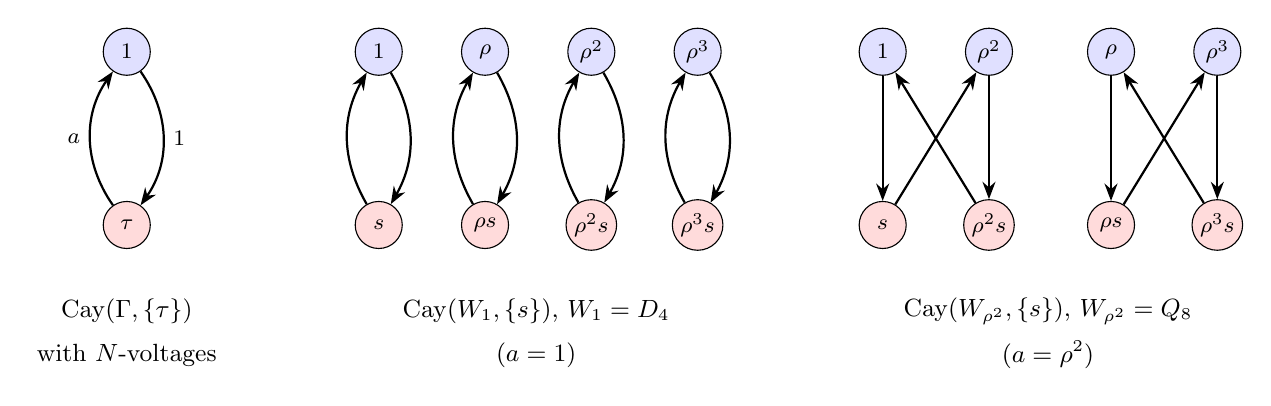
\begin{tikzpicture}[x=1cm,y=1cm]
% base graph
\node[bx] (b1) at (0,0) {$1$};
\node[rx] (bt) at (0,-2.2) {$\tau$};
\draw[ar] (b1) to[bend left=35] node[right,font=\footnotesize] {$1$} (bt);
\draw[ar] (bt) to[bend left=35] node[left,font=\footnotesize] {$a$} (b1);
\node[font=\small] at (0,-3.3) {$\Cay(\Gamma,\{\tau\})$};
\node[font=\small] at (0,-3.85) {with $N$-voltages};
% D4
\begin{scope}[shift={(3.2,0)}]
\foreach \k/\lab/\labs in {0/1/s,1/\rho/\rho s,2/\rho^2/\rho^2 s,3/\rho^3/\rho^3 s}{
  \node[bx] (u\k) at (1.35*\k,0) {$\lab$};
  \node[rx] (d\k) at (1.35*\k,-2.2) {$\labs$};
  \draw[ar] (u\k) to[bend left=30] (d\k);
  \draw[ar] (d\k) to[bend left=30] (u\k);
}
\node[font=\small] at (2.0,-3.3) {$\Cay(W_1,\{s\})$, $W_1=D_4$};
\node[font=\small] at (2.0,-3.85) {($a=1$)};
\end{scope}
% Q8
\begin{scope}[shift={(9.6,0)}]
\node[bx] (p0) at (0,0) {$1$};
\node[bx] (p2) at (1.35,0) {$\rho^2$};
\node[rx] (q0) at (0,-2.2) {$s$};
\node[rx] (q2) at (1.35,-2.2) {$\rho^2 s$};
\draw[ar] (p0) -- (q0);
\draw[ar] (q0) -- (p2);
\draw[ar] (p2) -- (q2);
\draw[ar] (q2) -- (p0);
\node[bx] (p1) at (2.9,0) {$\rho$};
\node[bx] (p3) at (4.25,0) {$\rho^3$};
\node[rx] (q1) at (2.9,-2.2) {$\rho s$};
\node[rx] (q3) at (4.25,-2.2) {$\rho^3 s$};
\draw[ar] (p1) -- (q1);
\draw[ar] (q1) -- (p3);
\draw[ar] (p3) -- (q3);
\draw[ar] (q3) -- (p1);
\node[font=\small] at (2.1,-3.3) {$\Cay(W_{\rho^2},\{s\})$, $W_{\rho^2}=Q_8$};
\node[font=\small] at (2.1,-3.85) {($a=\rho^2$)};
\end{scope}
\end{tikzpicture}
\caption{The Cayley digraph of $\Gamma=\{1,\tau\}$ with its $N$-voltages,
and its two derived graphs. Blue vertices lie over $1$ and red vertices
over $\tau$. The closed walk $1\to\tau\to1$ has net voltage $a$. It lifts
to closed walks when $a=1$ and to paths from $x$ to $x\rho^2$ when
$a=\rho^2$.}\label{fig:toy}
\end{figure}

\begin{example}[Unramified extensions]\label{ex:unramified}
Let $E/F$ be unramified of degree $n$, let $\tau$ be a generator of
$\Gamma$, and let $a=s_\tau^{\,n}\in F^\times$. By (W3) and the
isomorphism $H^2(\Gamma,E^\times)\cong F^\times/\Nm E^\times$ for cyclic
$\Gamma$ \cite[Ch.~VIII, \S4]{Se}, the class of $a$ generates
$F^\times/\Nm E^\times$. Since the norm group consists of the
elements whose valuation is divisible by $n$, the integer $m=\val_F(a)$ is
prime to $n$. Let $G$ be split, so that $\Gamma$ acts trivially on
$A=\Gh$, let $t\in\Gh$ be semisimple, and let
$\phi_t(x)=t^{\val_E(x)}$. Then $\phi_t$ is $\Gamma$-equivariant,
$T_{\phi_t}(\tau)=C_{\phi_t}=\Cent_{\Gh}(t)$, and~\eqref{eq:twistednorm}
reads
\[
c^{\,n}=t^{\,m},\qquad c\in\Cent_{\Gh}(t).
\]
A solution exists: $t$ lies in a maximal torus of $\Gh$, and complex tori
are divisible. So every $\phi_t$ extends to a cocycle of $W_{E/F}$, with
$f(s_\tau)=c$. The unramified parameters of $G$ are of this kind.
\end{example}

\begin{remark}[Balance]\label{rem:balance}
A gain function is \emph{balanced} if every closed walk has net gain~$1$
\cite{Za}. If the extension splits and the $s_t$ are chosen in the image
of a homomorphic section, then $\nu=1$ and~\eqref{eq:holonomy} says that
$\theta_c$ is balanced. In general, pull $\theta_c$ back along $p$ to a
gain function $p^*\theta_c$ on $\Cay(W,S)$. A closed walk at $1$ in
$\Cay(W,S)$ is spelled by some $r\in\rel$ with $\nu(r)=1$,
so~\eqref{eq:holonomy} implies that $p^*\theta_c$ is balanced. The cocycle
$f$ of Theorem~\ref{thm:graph} is then a \emph{potential} for
$p^*\theta_c$: along the edge from $w$ to $ws_t$ one has
$f(ws_t)=f(w)\cdot(p^*\theta_c)(w,s_t)$. Its values on the fiber $N$ over
the vertex $1$ are given by $\phi$. In these terms
Theorem~\ref{thm:graph} says that $\phi$ extends to a cocycle exactly when
some equivariant gain function $\theta_c$ on the base graph has a
pull-back which is balanced and admits a potential equal to $\phi$ on the
fiber over~$1$.
\end{remark}

\subsection{Running example: the graphs}\label{ss:run4}

\begin{example}[Running example, part 4]\label{ex:run4}
Keep the notation of Examples~\ref{ex:run1} to~\ref{ex:run3}. Take
$\overline{S}=\{\tau\}$ and $s_\tau=s$.

\smallskip\noindent\emph{(a) The base graph and its voltages.} The Cayley
digraph $\Cay(\Gamma,\{\tau\})$ is the directed $2$-cycle with edges
$1\to\tau$ and $\tau\to1$. For the section $s(\tau)=s$ the
$E^\times$-voltages of Proposition~\ref{prop:derived} are
\[
\nu_s(1,\tau)=s(1)\,s\,s(\tau)^{-1}=1,\qquad
\nu_s(\tau,\tau)=s(\tau)\,s\,s(1)^{-1}=s^2=3 .
\]
The free group $\fr$ is infinite cyclic, generated by the letter $\tau$,
and $\rel$ is generated by the word $\tau^2$, which spells the closed walk
$1\to\tau\to1$. Its net voltage is $\nu(\tau^2)=1\cdot3=3$. If the section
is changed to $s'(\tau)=ys$, the two voltages become $y^{-1}$ and $3y$
(switching by $\eta(\tau)=y$), and the net voltage is still $3$.

\smallskip\noindent\emph{(b) The derived graph.} The derived graph has
vertex set $\Gamma\times E^\times$ and edges $(1,x)\to(\tau,x)$ and
$(\tau,x)\to(1,3x)$. Under $(g,x)\mapsto x\,s(g)$ it becomes
$\Cay(W,\{s\})$, with edges $x\to xs$ and $xs\to xs^2=3x$. The connected
component of $x$ is the two-way infinite directed path
\[
\cdots\to 3^{-1}x\to 3^{-1}xs\to x\to xs\to 3x\to 3xs\to 9x\to\cdots,
\]
which covers the $2$-cycle infinitely many times. The components
correspond to the elements of
$E^\times/\nu(\rel)=E^\times/3^{\Z}\cong\cO^\times$, as in
Proposition~\ref{prop:derived}(v). The graph is not connected because
$\{s\}$ does not generate $W$. The group $E^\times$ acts by left
multiplication, permuting the paths and translating each path by its
powers of $3$.

\smallskip\noindent\emph{(c) Gains and holonomy.} Let
$\phi:E^\times\to A$ have a $\Gamma$-invariant class and let
$c\in T_\phi(\tau)$. The gain function is $\theta_c(1,\tau)=c$ and
$\theta_c(\tau,\tau)=\act{\tau}{c}$, so the holonomy around the $2$-cycle
is $\theta_c(\tau^2)=c\cdot\act{\tau}{c}$. Theorem~\ref{thm:graph}
(equivalently Corollary~\ref{cor:cyclic} with $n=2$ and $a=3$) says that
$\phi$ extends, with $f(s)=c$, if and only if
\[
\underbrace{c\cdot\act{\tau}{c}}_{\text{holonomy of }\theta_c}
\;=\;\phi(\underbrace{3}_{\text{net voltage}}).
\]
This is~\eqref{eq:run-c}. For $\Th$ the holonomy is $c\,c^{-1}=1$ for
every $c$. For $\SL_2(\C)$ and $\phi_{2,z}$ the holonomy is
$c_t^{\,2}=-1$ for every admissible $c$. In both cases the holonomy does
not depend on the choice of gains, and the question is only whether
$\phi(3)$ equals it.

\smallskip\noindent\emph{(d) The potential.} Let $\phi=\phi_{2,-1}$ and
$c=w_0$. The cocycle $f=f_1$ of Example~\ref{ex:run3}(b) labels the
vertices of $\Cay(W,\{s\})$, and along each edge $w\to ws$ the label is
multiplied on the right by the gain $w_0$
(Remark~\ref{rem:balance}). On the component of $1$ the labels are
\[
f(3^m)=(-1)^m,\qquad f(3^ms)=(-1)^mw_0 ,
\]
which under $Q_8\subset\SL_2(\C)$ is the periodic sequence
$\dots,1,j,-1,-j,1,j,\dots$ (Figure~\ref{fig:run}). So $f$ wraps the
infinite path around the directed $4$-cycle $1\to j\to-1\to-j\to1$, which
is a component of $\Cay(Q_8,\{j\})$ in Figure~\ref{fig:toy}. On the
component of $x$ all labels are multiplied on the left by $\phi(x)$. For
$\phi_{2,1}$ no such labeling exists: going twice around the base
$2$-cycle multiplies the label by $w_0^2=-1$, but the lifted walk goes
from $x$ to $3x$, where the label must be $\phi(3x)=\phi(x)$.
\end{example}

\begin{figure}[ht]
\centering
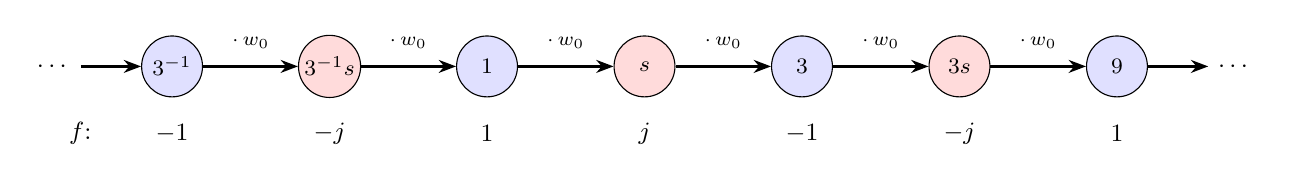
\begin{tikzpicture}[x=1cm,y=1cm]
\node[font=\small] (l) at (-1.5,0) {$\cdots$};
\node[bx,minimum size=22pt] (a0) at (0,0) {$3^{-1}$};
\node[rx,minimum size=22pt] (a1) at (2,0) {$3^{-1}s$};
\node[bx,minimum size=22pt] (a2) at (4,0) {$1$};
\node[rx,minimum size=22pt] (a3) at (6,0) {$s$};
\node[bx,minimum size=22pt] (a4) at (8,0) {$3$};
\node[rx,minimum size=22pt] (a5) at (10,0) {$3s$};
\node[bx,minimum size=22pt] (a6) at (12,0) {$9$};
\node[font=\small] (r) at (13.5,0) {$\cdots$};
\draw[ar] (l)--(a0); \draw[ar] (a0)--(a1); \draw[ar] (a1)--(a2);
\draw[ar] (a2)--(a3); \draw[ar] (a3)--(a4); \draw[ar] (a4)--(a5);
\draw[ar] (a5)--(a6); \draw[ar] (a6)--(r);
\foreach \n/\lab in {a0/-1,a1/-j,a2/1,a3/j,a4/-1,a5/-j,a6/1}{
  \node[font=\small] at ([yshift=-0.85cm]\n) {$\lab$};
}
\node[font=\small,anchor=east] at (-0.9,-0.85) {$f$:};
\foreach \x in {1,3,5,7,9,11}{
  \node[font=\scriptsize] at (\x,0.3) {$\cdot\,w_0$};
}
\end{tikzpicture}
\caption{The component of $1$ in $\Cay(W,\{s\})$ for $W=W_{\Q_3(i)/\Q_3}$,
with the values of the cocycle $f=f_1$ extending $\phi_{2,-1}$, written in
$Q_8\subset\SL_2(\C)$ with $j=w_0$. Blue vertices lie in $E^\times$ (over
$1\in\Gamma$) and red vertices in $E^\times s$ (over $\tau$). Each edge
multiplies the label by the gain $w_0$; two steps multiply the vertex by
the net voltage $3$ and the label by the holonomy
$w_0^2=-1=\phi_{2,-1}(3)$.}\label{fig:run}
\end{figure}

\section{Topology and Langlands parameters}\label{sec:langlands}

So far all groups were discrete. The Weil group is a locally compact group
and Langlands parameters are continuous, so we record how the results
adapt.

\begin{proposition}\label{prop:cont}
Suppose $W$ is a topological group in which $N$ is an open subgroup, and
$A$ is a topological group on which $\Gamma$ acts. A cocycle
$f\in Z^1(W,A)$ is continuous if and only if $f|_N$ is continuous.
Consequently Theorems~\ref{thm:exact}, \ref{thm:main}
and~\ref{thm:graph}, Proposition~\ref{prop:fiber} and
Corollaries~\ref{cor:central} and~\ref{cor:cyclic} remain true when
$Z^1(W,A)$ and $\Hom(N,A)$ are replaced by their subsets of continuous
maps. The group $\Gamma=W/N$ is discrete and its cocycles are unrestricted.
\end{proposition}

\begin{proof}
$W$ is the disjoint union of the open sets $N\,s(g)$, and on $N\,s(g)$ the
cocycle is $x\,s(g)\mapsto f(x)\,f(s(g))$ by~\eqref{eq:fxw}. So $f$ is
continuous if and only if $f|_N$ is. The relation~\eqref{eq:cohom} does not
involve the topology. In each statement the cocycles of $W$ that occur are
built from, or restrict to, a homomorphism $\phi$ on $N$, so the
continuous versions follow.
\end{proof}

For $W=W_{E/F}$ the subgroup $E^\times$ is the image of the open subgroup
$W_E$ of $W_F$, so it is open and Proposition~\ref{prop:cont} applies.

\begin{remark}[Parameters]\label{rem:parameters}
Let $\LG=\Gh\rtimes\Gamma$ be the finite Galois form of the $L$-group
\cite{Bo}. By Lemma~\ref{lem:semidirect}, continuous cocycles
$f\in Z^1(W_{E/F},\Gh)$ are the same as continuous homomorphisms
$W_F\to\LG$ over $\Gamma$ which are trivial on $W_E^c$, that is, whose
restriction to $W_E$ has abelian image; and cohomologous cocycles
correspond to $\Gh$-conjugate homomorphisms. Langlands parameters satisfy
further conditions \cite[\S8]{Bo}, which are not studied here. In this
language Theorem~\ref{thm:main} answers the question: \emph{which
homomorphisms $E^\times\to\Gh$ occur as the restriction to $W_E$ of a
homomorphism $W_F\to\LG$ over $\Gamma$?} The group $E_\phi$ is the
stabilizer of $\phi$ in $\LG$.
\end{remark}

\begin{example}\label{ex:langlands}
(a) For the norm-one torus $T$ of a quadratic extension,
Example~\ref{ex:torus2} with continuous characters gives
$H^1_{\mathrm{cont}}(W_{E/F},\Th)\cong\Hom_{\mathrm{cont}}(T(F),\C^\times)$.

(b) In Example~\ref{ex:dihedral}, a continuous character $\chi$ of
$E^\times$ with $\chi\circ\tau=\chi^{-1}\neq\chi$ gives a parameter
$W_F\to\SL_2(\C)$ of $\PGL_2$ if and only if
$\chi|_{F^\times}=\omega_{E/F}$. When $\chi|_{F^\times}=1$ the induced
representation has determinant $\omega_{E/F}$; it is a parameter with
values in $\GL_2(\C)$ but not in $\SL_2(\C)$.

(c) In Example~\ref{ex:unramified} the homomorphisms $\phi_t$ and the
cocycles extending them are continuous for the discrete topology on $\Gh$,
hence also for its complex topology.
\end{example}

\subsection{Running example: the parameters}\label{ss:run5}

\begin{example}[Running example, part 5]\label{ex:run5}
In the model of Example~\ref{ex:run1}, give $E^\times$ its $3$-adic
topology and $W=E^\times\sqcup E^\times s$ the topology in which
$E^\times$ is open. The characters $\chi_{k,z}$ are continuous, because
they are trivial on the open subgroup $U^1$. By
Proposition~\ref{prop:cont}, all cocycles found in
Example~\ref{ex:run3} are continuous. Composing with $W_F\to W_{E/F}$, we
obtain the following.

\smallskip\noindent\emph{(a)} For the norm-one torus $T$ of
$\Q_3(i)/\Q_3$, the tamely ramified part of
$H^1_{\mathrm{cont}}(W,\Th)$ consists of the four classes over
$\chi_{0,1},\chi_{2,1},\chi_{4,1},\chi_{6,1}$. They correspond to the four
characters of $T(\Q_3)=E^1$ that are trivial on $E^1\cap U^1$.

\smallskip\noindent\emph{(b)} The homomorphism $f_1:W\to\SL_2(\C)$ with
image $Q_8$ is a continuous, irreducible, tamely ramified parameter of
$\PGL_2$ over $\Q_3$. It is the only class of homomorphisms
$W\to\SL_2(\C)$ whose restriction to $E^\times$ is conjugate to
$\diag(\chi_{2,-1},\chi_{2,-1}^{-1})$. Its restriction to
$\Q_3^\times\subset E^\times$ is $\chi_{2,-1}|_{\Q_3^\times}$, which sends
$3$ to $-1$ and is trivial on units: this is the unramified quadratic
character $\omega_{E/F}$, as required by Example~\ref{ex:dihedral}.

\smallskip\noindent\emph{(c)} For $\chi_{2,1}$, which is trivial on
$\Q_3^\times$, the induced representation has values in $\GL_2(\C)$, image
the dihedral group of order $8$, and determinant equal to the non-trivial
character of $\Gamma$. It is a parameter of $\GL_2$ but not of $\PGL_2$.
\end{example}

\section{Questions}\label{sec:questions}

\begin{question}\label{q:nonab}
Theorem~\ref{thm:exact} holds for an arbitrary normal subgroup $N$
\cite[Ch.~I, \S5]{Se2}. If $N$ is not abelian, $\phi(N)$ is no longer
contained in $C_\phi$ and $\sigma$ is no longer a cocycle. Statement (e) of
Theorem~\ref{thm:main} still makes sense. What is the right obstruction
class?
\end{question}

\begin{question}\label{q:roots}
Let $W=W_{E/F}$ and $A=\Gh$, and let $\phi$ take values in a maximal torus
of $\Gh$. Then $C_\phi$ is a reductive group, possibly disconnected.
Describe $\kappa_\phi$ and $\partial\phi$ in terms of the root datum of
$G$ and of characters of $E^\times$, generalizing
Example~\ref{ex:dihedral}.
\end{question}

\begin{question}\label{q:continue}
For abelian $A$ the sequence of Corollary~\ref{cor:central}(iii) continues
with the inflation map $H^2(\Gamma,A)\to H^2(W,A)$. Is there a useful
non-abelian continuation, with $H^2(\Gamma,C_\phi,\kappa_\phi)$ in place of
$H^2(\Gamma,A)$?
\end{question}

\begin{question}\label{q:harmonic}
The covering $\Cay(W,S)\to\Cay(\Gamma,\overline{S})$ is a harmonic
morphism (Remark~\ref{rem:harmonic}). Is there an analog of
Theorem~\ref{thm:graph} for harmonic morphisms which are not coverings,
for instance for quotients of a Cayley graph by a group action which is
not free?
\end{question}

\section*{Acknowledgments}
\addcontentsline{toc}{section}{Acknowledgments}

The first author thanks A.~DuPre for conversations on $H^2$ at the time
of the original manuscript.

AI systems were used in preparing this revision, as follows.
\begin{itemize}[itemsep=2pt]
\item \emph{Gemini (Google)}, called ``Carbon'' in the first author's notes,
acted as referee of the original manuscript. Its report identified the
false identification of $\Gamma$-invariant classes with classes of
$\Gamma$-equivariant homomorphisms, the over-constrained hypothesis on the
section, inconsistent conjugation conventions, and a list of misprints,
and it proposed formula~\eqref{eq:fc}.
\item \emph{Claude (Anthropic)}, the second author, prepared this revision
under the first author's direction: it checked the referee's report, rewrote the text, found that
the obstruction must be taken in the centralizer $C_\phi$ and not in $A$
(Theorem~\ref{thm:main}, Example~\ref{ex:needed}), added
Proposition~\ref{prop:fiber}, the examples, Section~\ref{sec:graph},
Section~\ref{sec:langlands} and the glossary, and wrote the verification
script.
\end{itemize}
The first author wrote the original manuscript, directed the revision,
and is responsible for the content. Further details of the AI
usage, the comparison with the original manuscript, the response to the
referee, and the list of sources consulted and not consulted are in the
revision log, \texttt{revision-log.tex}, in the folder \texttt{infres} of
the repository \url{https://github.com/wdjoyner/alg-graph-thry}.

\section*{Glossary}
\addcontentsline{toc}{section}{Glossary}

Each entry is meant to be read on its own. Throughout, $\Gamma$ is a
group, $A$ is a group on which $\Gamma$ acts, and $1\to N\to W\to\Gamma\to1$
is an extension with $N$ abelian. The ``toy example'' is $N=\Z/4$ with
generator $\rho$, $\Gamma=\{1,\tau\}$ acting on $N$ by inversion, and
$A=Q_8=\{\pm1,\pm i,\pm j,\pm k\}$ with trivial action.

\begin{description}[itemsep=3pt,leftmargin=1.5em,style=unboxed]
\item[Abelianization.] The largest abelian quotient of a group, obtained
by dividing by the subgroup generated by all commutators $xyx^{-1}y^{-1}$.
For a topological group one divides by the closure of that subgroup. The
abelianization of the Weil group $W_E$ is $E^\times$.

\item[Balanced gain function.] A gain function on a graph for which the
net gain around every closed walk is the identity. Equivalently, the gains
come from a labeling of the vertices (a potential): the gain of an edge is
the ``ratio'' of the labels at its two ends. On a tree every gain function
is balanced; on a cycle a gain function is balanced exactly when the
product of the gains around the cycle is~$1$.

\item[Bouquet.] A graph with a single vertex and a set of loops. Every
Cayley digraph of a group with generating set $\overline{S}$ covers the
bouquet with one loop for each element of $\overline{S}$.

\item[Cayley digraph $\Cay(\Gamma,\overline{S})$.] The directed graph with
one vertex for each element $g$ of the group $\Gamma$ and one edge from
$g$ to $gt$ for each $t$ in a chosen subset $\overline{S}$. It is connected
exactly when $\overline{S}$ generates $\Gamma$. For a cyclic group of
order $n$ and one generator it is a directed $n$-cycle.

\item[Central homomorphism.] A homomorphism $\phi:N\to A$ whose image lies
in the center of $A$. Every homomorphism into an abelian group is central.
For central homomorphisms, having a $\Gamma$-invariant conjugacy class is
the same as being $\Gamma$-equivariant.

\item[Centralizer $C_\phi$.] For a homomorphism $\phi:N\to A$, the
subgroup of all elements of $A$ that commute with every $\phi(x)$. In the
toy example with $\phi(\rho)=i$ it is $\{\pm1,\pm i\}$. For
$\phi=\diag(\chi,\chi^{-1})$ with values in $\SL_2(\C)$ and $\chi^2\neq1$
it is the diagonal torus.

\item[Closed walk.] A walk in a graph that ends at the vertex where it
starts. In a Cayley digraph, the closed walks based at the identity are
spelled by exactly those words in the generators that equal the identity
in the group.

\item[Coboundary.] A cocycle of the simplest kind, obtained from a
cochain of one degree lower. A $1$-coboundary of $\Gamma$ in $A$ is a map
$g\mapsto a^{-1}\,\act{g}{a}$ for a fixed $a\in A$. Two cocycles that
differ by a coboundary (in the appropriate twisted sense, when $A$ is not
abelian) are cohomologous.

\item[Cohomologous cocycles.] Two $1$-cocycles $f,f'$ of a group $G$ in
$A$ are cohomologous if $f'(g)=a^{-1}f(g)\,\act{g}{a}$ for a fixed
$a\in A$. When $G$ acts trivially on $A$, this means that $f$ and $f'$ are
homomorphisms conjugate under $A$.

\item[Cohomology set $H^1(G,A)$.] The set of $1$-cocycles of $G$ in $A$
modulo the relation of being cohomologous. It is a group when $A$ is
abelian, and otherwise only a set with a distinguished point, the class of
the constant cocycle~$1$. When $G$ acts trivially it is the set of
conjugacy classes of homomorphisms $G\to A$.

\item[Covering map of graphs.] A map of graphs which sends vertices to
vertices and edges to edges, and which near each vertex is a bijection
between the edges at that vertex and the edges at its image. The quotient
of a graph by a group acting freely is a covering map. The $n$-cycle
covers the loop, and a $2n$-cycle covers an $n$-cycle.

\item[Defining relators.] For a group $\Gamma$ with generating set
$\overline{S}$, a set of words in the generators which equal the identity
in $\Gamma$ and from which every such word follows, by multiplying
conjugates of them and their inverses. For the cyclic group of order $n$
with generator $\tau$, the single relator $\tau^n$ suffices. For the Klein
four-group with generators $a,b$ one may take $a^2$, $b^2$ and
$aba^{-1}b^{-1}$.

\item[Derived graph.] The covering graph built from a voltage assignment
$\nu$ with values in a group $K$. Its vertices are pairs (vertex, element
of $K$), and an edge from $v$ to $v'$ with voltage $\nu(e)$ gives edges
from $(v,k)$ to $(v',k\,\nu(e))$ for all $k\in K$. A loop with voltage a
generator of $\Z/n$ has the $n$-cycle as derived graph. The Cayley digraph
of an extension $W$ is a derived graph of the Cayley digraph of the
quotient $\Gamma$.

\item[Dihedral parameter.] A two-dimensional representation of the Weil
group of $F$ induced from a character $\chi$ of $E^\times$, where $E/F$ is
a quadratic extension. On $E^\times$ it is $\diag(\chi,\chi\circ\tau)$,
and an element over the non-trivial automorphism $\tau$ acts by an
anti-diagonal matrix.

\item[Digraph.] A directed graph: a set of vertices and a set of edges,
each edge having a tail and a head. Loops and several edges between the
same two vertices are allowed in this note.

\item[Dual group $\Gh$.] The complex reductive group whose root datum is
obtained from that of a reductive group $G$ by exchanging roots and
coroots. The dual group of $\GL_n$ is $\GL_n(\C)$, that of $\PGL_2$ is
$\SL_2(\C)$, that of $\SL_2$ is $\PGL_2(\C)$, and that of a torus is a
complex torus. A Galois group acts on $\Gh$; the action is trivial when
$G$ is split.

\item[Equivariant homomorphism.] A homomorphism $\phi:N\to A$ between
groups with $\Gamma$-action such that
$\phi(\act{g}{x})=\act{g}{\phi(x)}$ for all $g$ and $x$. This is stronger
than having a $\Gamma$-invariant conjugacy class.

\item[Exact sequence of pointed sets.] A sequence $X\to Y\to Z$ of sets
with base points in which the image of $X$ is the set of elements of $Y$
sent to the base point of $Z$. Unlike for groups, this gives no
information about the other fibers of $Y\to Z$; those are obtained by
twisting.

\item[Extension of groups.] A group $W$ with a normal subgroup $N$ and an
identification of $W/N$ with $\Gamma$, written $1\to N\to W\to\Gamma\to1$.
One says that $W$ is an extension of $\Gamma$ by $N$. The cyclic group of
order $8$, the dihedral group of order $8$ and the quaternion group are
all extensions of $\Z/2$ by $\Z/4$.

\item[Factor set.] For a section $s$ of an extension, the function
$\sigma(g,h)=s(g)s(h)s(gh)^{-1}$ with values in $N$. It measures the
failure of $s$ to be a homomorphism, and it is a $2$-cocycle. In the
quaternion group, as an extension of $\{1,\tau\}$ by $\langle i\rangle$
with $s(\tau)=j$, its only non-trivial value is
$\sigma(\tau,\tau)=j^2=-1$.

\item[Fiber.] The set of elements mapped to a given element by a map. For
the covering $\Cay(W,S)\to\Cay(\Gamma,\overline{S})$, the fiber over the
vertex $1$ is the subgroup $N$. For the restriction map
$H^1(W,A)\to H^1(N,A)$, the fiber over a class $[\phi]$ is the set of
classes of cocycles of $W$ whose restriction to $N$ is conjugate to
$\phi$.

\item[Free group.] The group of reduced words in a set of letters and
their inverses, with no relations other than $tt^{-1}=1$. Every group
generated by $\overline{S}$ is a quotient of the free group on
$\overline{S}$. The free group on one letter is $\Z$.

\item[Fundamental class.] The canonical generator $u_{E/F}$ of the cyclic
group $H^2(\Gal(E/F),E^\times)$, of order $[E:F]$, given by local class
field theory. It is the class of the relative Weil group as an extension
of $\Gal(E/F)$ by $E^\times$. For a quadratic extension it is the
non-trivial element of $F^\times/\Nm E^\times$.

\item[Gain function.] An assignment of a group element to each edge of a
directed graph, with the convention that traversing the edge backward
contributes the inverse element. Also called a voltage assignment. In
this note the gains $\theta_c(g,t)=\act{g}{c(t)}$ on the Cayley digraph of
$\Gamma$ take values in $A$.

\item[$\Gamma$-group.] A group $A$ together with an action of $\Gamma$ by
group automorphisms, written $\act{g}{a}$. A $\Gamma$-module is an abelian
$\Gamma$-group. Any group is a $\Gamma$-group for the trivial action.

\item[Harmonic morphism.] A map of graphs sending vertices to vertices and
edges to edges or vertices, such that at each vertex the number of edges
mapping onto a given edge at the image vertex does not depend on that
edge. Covering maps are the harmonic morphisms for which this number is
always~$1$ and no edge is collapsed to a vertex.

\item[Holonomy.] The net gain of a gain function around a closed walk. It
measures what is picked up on returning to the starting vertex: it is
trivial for every closed walk exactly when the gain function is balanced.
In this note the holonomy of the gain function $\theta_c$ around a relator
$r$ of $\Gamma$ is required to equal $\phi(\nu(r))$, where $\nu(r)$ is the
net $N$-voltage of the same closed walk. In the toy example the only
relator is $\tau^2$, the holonomy is $c^2=-1$ for $c\in\{\pm j,\pm k\}$,
and the net voltage is $s^2$.

\item[Inflation.] The map $H^1(\Gamma,A)\to H^1(W,A)$ which composes a
cocycle of the quotient $\Gamma$ with the projection $W\to\Gamma$. For
trivial actions it sends a homomorphism $\Gamma\to A$ to the homomorphism
$W\to\Gamma\to A$. It is always injective.

\item[Inner automorphism; outer automorphism group.] The inner
automorphism $\Int(c)$ of a group $C$ is conjugation $z\mapsto czc^{-1}$.
The inner automorphisms form a normal subgroup $\Int(C)$ of $\Aut(C)$,
isomorphic to $C$ modulo its center, and $\Out(C)=\Aut(C)/\Int(C)$. For an
abelian group $\Out(C)=\Aut(C)$.

\item[Inner form.] A reductive group over $F$ which becomes isomorphic to
a given one over the algebraic closure by an isomorphism that differs from
its Galois conjugates by inner automorphisms. The multiplicative group of
a quaternion division algebra is an inner form of $\GL_2$. Inner forms
have the same dual group with the same Galois action.

\item[Invariant class.] A conjugacy class of homomorphisms $N\to A$ which
is mapped to itself by every element of $\Gamma$. The homomorphisms in it
need not be equivariant: in the toy example the class of $\phi$ with
$\phi(\rho)=i$ is invariant, since $\tau$ sends $\phi$ to its conjugate by
$j$, but it contains no equivariant homomorphism.

\item[Kernel (band).] A homomorphism $\kappa:\Gamma\to\Out(C)$. It is an
``action up to inner automorphisms'' of $\Gamma$ on a group $C$, and it is
the datum needed to define $H^2$ with coefficients in a non-abelian
group. Every extension of $\Gamma$ by $C$ has a kernel, given by
conjugation by lifts of elements of $\Gamma$. The word ``kernel'' here has
nothing to do with the kernel of a homomorphism.

\item[$L$-group.] The semidirect product $\LG=\Gh\rtimes\Gamma$ of the
complex dual group of a reductive group $G$ with a Galois group acting on
it. For a split group it is the direct product $\Gh\times\Gamma$.

\item[Langlands parameter.] A continuous homomorphism from the Weil group
(or Weil--Deligne group) of $F$ to the $L$-group which is compatible with
the projections to the Galois group and satisfies additional conditions,
taken up to conjugation by $\Gh$. For $\GL_n$ these are the
$n$-dimensional Frobenius-semisimple representations of the Weil--Deligne
group.

\item[Monodromy.] For a covering of graphs, the rule which assigns to
each closed walk in the base the way its lifts permute a fiber. For the
covering $\Cay(W,S)\to\Cay(\Gamma,\overline{S})$ it is the homomorphism
$\nu$ from the group of relations of $\Gamma$ to $N$: the lift of the
closed walk spelled by $r$, starting at the vertex $x$, ends at
$x\,\nu(r)$.

\item[Net voltage, net gain.] The ordered product of the voltages (gains)
of the edges of a walk, with inverses for edges traversed backward.

\item[Neutral class.] A class in $H^2(\Gamma,C,\kappa)$ containing a
cocycle of the form $(1,\beta)$. In terms of extensions of $\Gamma$ by
$C$, the neutral classes are the classes of split extensions. For abelian
$C$ only the trivial class is neutral. For non-abelian $C$ there may be
several neutral classes, or none.

\item[Norm-one torus.] For a quadratic extension $E/F$, the algebraic
torus over $F$ whose group of $F$-points is $E^1$, the elements of
$E^\times$ of norm $1$. Its dual group is $\C^\times$, on which the
non-trivial element of $\Gal(E/F)$ acts by inversion.

\item[Obstruction class $\partial\phi$.] The class in
$H^2(\Gamma,C_\phi,\kappa_\phi)$ attached to a homomorphism $\phi:N\to A$
with invariant class. It is the class of the stabilizer extension $E_\phi$
divided by the image under $\phi$ of the class of $W$. It is neutral
exactly when $\phi$ is the restriction of a $1$-cocycle of $W$. In the toy
example it is $-\phi(a)^{-1}\in\{\pm1\}$, where $a=s^2$.

\item[$1$-cocycle.] A map $f:G\to A$ with
$f(gh)=f(g)\,\act{g}{f(h)}$. When $G$ acts trivially on $A$ it is a
homomorphism. In general it is the first component of a homomorphism
$G\to A\rtimes G$ whose second component is the identity. For
$G=\{1,\tau\}$ a cocycle is an element $c=f(\tau)$ with
$c\,\act{\tau}{c}=1$.

\item[Pointed set.] A set with a chosen element, the base point. Maps of
pointed sets preserve base points.

\item[Potential.] A labeling of the vertices of a graph by elements of a
group which produces a given gain function: the label at the head of each
edge is the label at its tail times the gain of the edge. A gain function
has a potential exactly when it is balanced. A cocycle of $W$ is a
potential for a gain function on the Cayley digraph of $W$.

\item[Quadratic character $\omega_{E/F}$.] For a quadratic extension
$E/F$ of local fields, the character of $F^\times$ of order $2$ whose
kernel is the group of norms from $E^\times$.

\item[Reciprocity map.] The isomorphism of local class field theory
between $E^\times$ and the abelianization of the Weil group $W_E$.

\item[Relations, group of.] For a group $\Gamma$ with generating set
$\overline{S}$, the kernel $\rel$ of the natural map from the free group
on $\overline{S}$ onto $\Gamma$: the words which equal the identity in
$\Gamma$. It is the same as the set of closed walks at the identity in the
Cayley digraph, up to backtracking.

\item[Relative Weil group $W_{E/F}$.] The quotient of the Weil group
$W_F$ by the closure of the commutator subgroup of $W_E$. It is an
extension of $\Gal(E/F)$ by $E^\times$. For $\C/\R$ it is the group
$\C^\times\sqcup\C^\times j$ inside the quaternions, with $j^2=-1$ and
$jzj^{-1}=\overline{z}$.

\item[Restriction.] The map $H^1(W,A)\to H^1(N,A)$ which restricts a
cocycle of $W$ to the subgroup $N$. Its image consists of
$\Gamma$-invariant classes.

\item[Section.] A map $s:\Gamma\to W$ with $p\circ s$ the identity and
$s(1)=1$, where $p:W\to\Gamma$ is the projection. It is a choice of coset
representatives for $N$ in $W$ and need not be a homomorphism.

\item[Semidirect product $A\rtimes\Gamma$.] The set $A\times\Gamma$ with
multiplication $(a,g)(b,h)=(a\,\act{g}{b},gh)$. The dihedral group of
order $8$ is $\Z/4\rtimes\Z/2$ for the action by inversion.

\item[Split extension.] An extension $1\to N\to W\to\Gamma\to1$ for which
some section is a homomorphism; then $W\cong N\rtimes\Gamma$. The dihedral
group of order $8$ is a split extension of $\Z/2$ by $\Z/4$, and the
quaternion group is a non-split one. The relative Weil group $W_{E/F}$ is
not split when $E\neq F$.

\item[Springer $2$-cocycle.] A pair $(u,\beta)$, where the $\beta(g)$ are
automorphisms of $C$ and $u(g,h)\in C$, such that
$\beta(g)\beta(h)=\Int(u(g,h))\beta(gh)$ and
$u(g,h)u(gh,k)=\beta(g)(u(h,k))u(g,hk)$. It is the data produced by a
set-theoretic section $e$ of an extension of $\Gamma$ by $C$: $\beta(g)$
is conjugation by $e(g)$ and $u(g,h)=e(g)e(h)e(gh)^{-1}$. For abelian $C$
it is an ordinary $2$-cocycle together with the action of $\Gamma$.

\item[Stabilizer extension $E_\phi$.] The subgroup of $A\rtimes\Gamma$
fixing a homomorphism $\phi:N\to A$. When the class of $\phi$ is
invariant, it is an extension of $\Gamma$ by the centralizer $C_\phi$. In
the toy example with $\phi(\rho)=i$ it consists of the pairs $(z,1)$ and
$(zj,\tau)$ with $z\in\{\pm1,\pm i\}$.

\item[Switching.] The change of a voltage assignment $\nu$ produced by a
function $\eta$ on the vertices: the voltage of an edge from $v$ to $v'$
becomes $\eta(v)\,\nu(e)\,\eta(v')^{-1}$. Switching does not change net
voltages of closed walks up to conjugation, and it does not change the
derived graph up to isomorphism. Changing the section of an extension
switches the associated voltages.

\item[Transgression.] In the five-term exact sequence for abelian
coefficients, the map $H^1(N,A)^\Gamma\to H^2(\Gamma,A^N)$. With the
conventions of this note, and $N$ acting trivially on $A$, it is
$\phi\mapsto-\phi_*[\sigma]$: apply $\phi$ to a factor set of the
extension and invert.

\item[Transporter $T_\phi(g)$.] The set of $b\in A$ with
$b\,\act{g}{\phi(x)}\,b^{-1}=\phi(\act{g}{x})$ for all $x\in N$. It is
non-empty for all $g$ exactly when the class of $\phi$ is invariant, and
it is then a coset of the centralizer $C_\phi$. In the toy example with
$\phi(\rho)=i$, $T_\phi(\tau)=\{\pm j,\pm k\}$.

\item[Twisted norm.] For a cyclic group generated by $\tau$ of order $n$
acting on $A$, the product
$c\cdot\act{\tau}{c}\cdots\act{\tau^{n-1}}{c}$. For abelian $A$ it is the
usual norm. For a trivial action it is $c^n$.

\item[Twisting.] The passage from a $\Gamma$-group to the same group with
the action modified by a cocycle $f$: the new action of $g$ is
$z\mapsto f(g)\,\act{g}{z}\,f(g)^{-1}$. It is used to describe the fibers
of maps between non-abelian cohomology sets other than the fiber of the
base point.

\item[Unramified.] An extension $E/F$ of $p$-adic fields is unramified if
a uniformizer of $F$ remains a uniformizer of $E$. Such an extension is
cyclic, generated by the Frobenius automorphism. A character or parameter
is unramified if it is trivial on the units, respectively on the inertia
subgroup.

\item[Voltage assignment.] A gain function; the term is used when the
purpose is to construct a covering graph (the derived graph). In this
note the voltages $\nu_s(g,t)=s(g)s_ts(gt)^{-1}$ on the Cayley digraph of
$\Gamma$ take values in $N$.

\item[Walk.] A sequence of edges of a graph, each traversed forward or
backward, in which each edge starts where the previous one ends. In a
Cayley digraph a walk from the identity is the same as a word in the
generators and their inverses.

\item[Weil group $W_F$.] For a $p$-adic field $F$, the subgroup of the
absolute Galois group consisting of the elements that act on the residue
field of the algebraic closure by an integral power of Frobenius, with the
topology in which the inertia subgroup is open. Its abelianization is
$F^\times$.
\end{description}

\begin{thebibliography}{99}

\bibitem[AT]{AT} E.~Artin and J.~Tate, \emph{Class field theory},
W.~A.~Benjamin, 1968; reprinted by AMS Chelsea, 2009.

\bibitem[BN]{BN} M.~Baker and S.~Norine, Harmonic morphisms and
hyperelliptic graphs, \emph{Int.\ Math.\ Res.\ Not.\ IMRN} 2009, no.~15,
2914--2955.

\bibitem[Bo]{Bo} A.~Borel, Automorphic $L$-functions, in \emph{Automorphic
forms, representations and $L$-functions} (Corvallis, 1977), Proc.\ Sympos.\
Pure Math.\ 33, Part~2, Amer.\ Math.\ Soc., 1979, 27--61.

\bibitem[Bor]{Bor} M.~Borovoi, Abelianization of the second nonabelian
Galois cohomology, \emph{Duke Math.\ J.} 72 (1993), 217--239.

\bibitem[Gi]{Gi} J.~Giraud, \emph{Cohomologie non ab\'elienne},
Grundlehren der math.\ Wissenschaften 179, Springer-Verlag, 1971.

\bibitem[GT]{GT} J.~L.~Gross and T.~W.~Tucker, \emph{Topological graph
theory}, Wiley, 1987.

\bibitem[HS]{HS} G.~Hochschild and J.-P.~Serre, Cohomology of group
extensions, \emph{Trans.\ Amer.\ Math.\ Soc.} 74 (1953), 110--134.

\bibitem[La]{La} R.~P.~Langlands, Representations of abelian algebraic
groups, \emph{Pacific J.\ Math.} 181 (1997), no.~3, 231--250.

\bibitem[ML]{ML} S.~Mac~Lane, \emph{Homology}, Grundlehren der math.\
Wissenschaften 114, Springer-Verlag, 1963.

\bibitem[Se]{Se} J.-P.~Serre, \emph{Local fields}, Graduate Texts in
Math.\ 67, Springer-Verlag, 1979.

\bibitem[Se2]{Se2} J.-P.~Serre, \emph{Galois cohomology}, Springer-Verlag,
1997.

\bibitem[Spr]{Spr} T.~A.~Springer, Nonabelian $H^2$ in Galois cohomology,
in \emph{Algebraic groups and discontinuous subgroups} (Boulder, 1965),
Proc.\ Sympos.\ Pure Math.\ 9, Amer.\ Math.\ Soc., 1966, 164--182.

\bibitem[Ta]{Ta} J.~Tate, Number theoretic background, in
\emph{Automorphic forms, representations and $L$-functions} (Corvallis,
1977), Proc.\ Sympos.\ Pure Math.\ 33, Part~2, Amer.\ Math.\ Soc., 1979,
3--26.

\bibitem[Za]{Za} T.~Zaslavsky, Biased graphs. I. Bias, balance, and gains,
\emph{J.\ Combin.\ Theory Ser.~B} 47 (1989), 32--52.

\end{thebibliography}

\end{document}
